\documentclass[11pt, a4paper]{report}
%-----------NORSK LaTeX--------------

% Denne pakken inkluderer skandinaviske bokstaver( æ, ø og å)
\usepackage[utf8]{inputenc}

% Denne pakken bruker norsk typesetting (innholdsliste osv.)
\usepackage[norsk]{babel}

%--------DOKUMENTOPPSETT------------

% Lar deg tilpasse layouten i prosjektet
\usepackage{fancyhdr}

% Definere egne farger 
\usepackage[usenames, dvipsnames]{color}

% Avstand på marger til sidene på arket
%\usepackage{geometry}

% Linker i dokumentet (figurer, seksjoner osv)
\usepackage[hidelinks]{hyperref}

% Kildeliste-setup
%\usepackage[natbibapa]{apacite} % For apalike eller apacite
\usepackage{natbib} % For Chicago, Vancover, Harvard Style, Nature Style osv

% Spacing mellom bokstaver
\usepackage{microtype}

% Laster inn forskjellige skrifttyper
\usepackage{uarial} % Arial
\usepackage[scaled]{helvet} % Helvetica
%\usepackage{tgbonum} % Usikker
%\usepackage{mathptmx} % Times New Roman
%\usepackage{lmodern} % Latin Modern
%\usepackage[charter]{mathdesign} % Charters
\usepackage[T1]{fontenc}

% Avsnitt mellom paragrafer
\usepackage{parskip}

% Linjeavstand i dokumentet
\usepackage{setspace}
\setlength{\parskip}{1em}

% Fet skrift på alle figurnr
\usepackage[labelfont=bf]{caption}
\usepackage{capt-of}
\usepackage{caption}
\usepackage{tikz}

\usepackage{chngcntr}
\counterwithin{figure}{chapter}
\counterwithin{table}{chapter}

% Definerer mellomrom mellom seksjons-, figur- og tabellnummer i innholdsliste til teksten begynner
\renewcommand{\numberline}[1]{#1 \,}

% Kan skrive i kolonner
\usepackage{multicol}

% For appendix
\usepackage{titletoc}
\usepackage{appendix}

%----------ANDRE PAKKER--------------

% Pakker fra AMS. Kan skrive matteformler
\usepackage{amsfonts, amssymb, amsthm}
\usepackage{mathtools}

% For grafikk (lime inn bilder, pdf-dokumenter)
\usepackage{graphicx}
\usepackage{float}
\usepackage{pdfpages}
\usepackage{subcaption}

% For inportering av csv-filer som tabeller. ( Ikkje i bruk)
%usepackage{csvsimple}

% Pakke for citations
%\usepackage{biblatex}
% Pakke for at url linker skal fungere i bl.a. referansar
\usepackage{url}

% Generere tekst
\usepackage{kantlipsum}

% Definere egne objekt
\usepackage{tikz}

% Lar deg lage lister på en mer oversiktlig måte
\usepackage[sharp]{easylist}

% Boks rundt tekst
\usepackage{fancyvrb}

% Test pakker
\usepackage{array}
\usepackage[margin=1in]{geometry} % Juster margene etter behov
\usepackage{titlesec}
\usepackage{tabularx}
\usepackage[table]{xcolor}
\usepackage{lastpage}

% For å kunne justere bilete
\usepackage{adjustbox}

% 
\usepackage{tocloft}


% Sider til SCD
\usepackage{afterpage}
\usepackage{adjustbox}
\usepackage{changepage}


%---------------------------------------------------

% Legger til bookmarks i pdf
\hypersetup{
    bookmarks=true, % Aktiver bokmerker
    bookmarksnumbered=true, % Inkluder nummer i bokmerker
    pdfstartview={FitH}, % Åpner PDF med passende bredde
    %colorlinks=true, % Farger lenker i stedet for å bruke bokser
    %linkcolor=blue, % Intern lenkefarge
    %filecolor=magenta, % Fil-lenkefarge
    %urlcolor=cyan % URL-lenkefarge
}



% Velger arial som skrifttype i dokumentet 
%\renewcommand{\rmdefault}{qpl} % 
%\renewcommand{\rmdefault}{phv} % Arial
\renewcommand*\familydefault{\sfdefault} % Helvetica(sans-serif)


% Definerer egne farger
\definecolor{mybla}{RGB}{25, 49, 90}
\definecolor{mylysbla}{RGB}{0, 136, 176}
\definecolor{renasysGreen}{RGB}{4, 255, 4}
\definecolor{purewhite}{RGB}{255,255,255}
\definecolor{lightgray}{gray}{0.8}
\definecolor{myblack}{gray}{0.1}

% Velger norsk språk på innholdsfortegnelse, figurliste, tabelliste og Referanseliste
% Legger disse så til i innholdsfortegnelsen.
\addto\captionsnorsk{\renewcommand{\contentsname}{Vedlegg}}
\addto\captionsnorsk{\renewcommand{\listfigurename}{Figurliste}}
\addto\captionsnorsk{\renewcommand{\listtablename}{Tabelliste}}
\addto\captionsnorsk{\renewcommand{\bibname}{Referansar}}
% Nynorsk!
\addto\captionsnynorsk{\renewcommand{\contentsname}{Innhaldsliste}} 
\addto\captionsnynorsk{\renewcommand{\listfigurename}{Figurliste}}
\addto\captionsnynorsk{\renewcommand{\listtablename}{Tabelliste}}
\addto\captionsnynorsk{\renewcommand{\bibname}{Referansar}}


% ----- Justering av avstander mellom chapter / section / subsection / subsubsection

% Justeringa av chapter, 
% første verdi : Horisontalverdi frå venstre marg
% Andre verdi : avstanden frå toppen av sida til tittelen
% Tredje verdi : Avstand til neste tekst
\titleformat{\chapter}[hang]
  {\normalfont\bfseries\LARGE}{\thechapter}{1em}{}
\titlespacing*{\chapter}{0pt}{-50pt}{0pt}

% Juster avstanden for \section
\titleformat{\section}
  {\normalfont\Large\bfseries}{\thesection}{1em}{}
\titlespacing*{\section}{0pt}{10pt}{10pt}

% Juster avstanden for \subsection
\titleformat{\subsection}
  {\normalfont\large\bfseries}{\thesubsection}{1em}{}
\titlespacing*{\subsection}{0pt}{10pt}{10pt}

% Juster avstanden for \subsubsection om nødvendig
\titleformat{\subsubsection}
  {\normalfont\normalsize\bfseries}{\thesubsubsection}{1em}{}
\titlespacing*{\subsubsection}{0pt}{10pt}{10pt}

% ------------------- jusetring av lister ------------------

% Denne vil endre skriftstørrelse ...
% Legg til \hfill før LARGE om overskrifta skal sentrerest
\renewcommand{\cfttoctitlefont}{\LARGE\bfseries}
\renewcommand{\cftaftertoctitle}{}
\renewcommand{\cftloftitlefont}{\LARGE\bfseries}
\renewcommand{\cftafterloftitle}{}
\renewcommand{\cftlottitlefont}{\LARGE\bfseries}
\renewcommand{\cftafterlottitle}{}

% Avstand mellom toppen av sida og ned til overskrifta t.d. innhaldsliste
\setlength{\cftbeforetoctitleskip}{-20pt}  % Adjust the value as needed, negative reduces the space
\setlength{\cftbeforeloftitleskip}{-20pt}  % Adjust the value as needed
\setlength{\cftbeforelottitleskip}{-20pt}  % Adjust the value as needed

% Avstand mellom Overskrift og kapittel
\setlength{\cftaftertoctitleskip}{15pt}
\setlength{\cftafterloftitleskip}{15pt}
\setlength{\cftafterloftitleskip}{15pt}


% -------------------------------------------------------------

% Her definerer ein pagestylen til hovud opplegget
\fancypagestyle{fancy}{
  % Clear the header and footer
  \fancyhf{}
  % Set the right side of the footer to be the location of the page number
  \fancyfoot[R]{Side \thepage\ av~\pageref{LastPage}} % Her sett ein fra side til side
  \renewcommand{\headrulewidth}{0pt} % Remove header line
  \renewcommand{\footrulewidth}{0pt} % Remove footer line
}

% Her definerer ein pagestylen til dei sidene som skal ha romartall
\fancypagestyle{romanpages}{
  % Clear the header and footer
  \fancyhf{}
  % Set the right side of the footer to be the location of the page number
  \fancyfoot[R]{\thepage}
  \renewcommand{\headrulewidth}{0pt} % Remove header line
  \renewcommand{\footrulewidth}{0pt} % Remove footer line
}


% ------ Justering av avstander i dokumentet for itemize ---------------------

\let\olditemize\itemize
\renewcommand{\itemize}{
  \olditemize
  \setlength{\itemsep}{-10pt} 
}

% ------ Justering av avstander i dokumentet for enumerable ---------------------

% Save the original definition of enumerate
\let\oldenumerate\enumerate

% Redefine the enumerate to adjust spacing
\renewcommand{\enumerate}{
  \oldenumerate
  \setlength{\itemsep}{-7pt}  % Adjust this value as needed
}



% Stil for referansar
\bibliographystyle{unsrt}


\begin{document} % Dokument start

\newgeometry{top=2.5cm,bottom=3cm,right=2.2cm,left=2.2cm}
% Førstesiden skal ha følgende marger.
\newgeometry{top=2.5cm,bottom=2.5cm,right=3cm,left=5cm}

% Ønsker ikke sidetall på denne siden.
\thispagestyle{empty}


% Legger inn banner
\begin{center}
	\begin{tikzpicture}[remember picture, overlay]
	\node [xshift=0cm, yshift=11.5cm] at (current page.center) 
	{
\includegraphics[width=\paperwidth]{Bilder/framsideNynorsk.png}};
	\end{tikzpicture}
\end{center}



\vspace{6cm}

{\fontsize{36}{50}\selectfont \textbf{\textcolor{mybla}{BACHELOROPPGÅVE}}} 
\newline
\newline
{\fontsize{26}{30}\selectfont \textcolor{mybla}{RA200 Sande}}

\vspace{1cm}
% Forfattarar
{\fontsize{26}{30}\selectfont \textbf{\textcolor{mylysbla}{Roar Bøyum}}}\\
{\fontsize{26}{30}\selectfont \textbf{\textcolor{mylysbla}{Vegard Aven Ullebø}}}\\
{\fontsize{26}{30}\selectfont \textbf{\textcolor{mylysbla}{Peter Søreide Skaar}}}\\ 


\vspace{1.3cm}


\setstretch{0.7}

{\fontsize{20}{20}\selectfont\textcolor{mylysbla}{Automatisering med robotikk}} 

\vspace{-0.4cm}
{\fontsize{20}{20}\selectfont\textcolor{mylysbla}{Fakultet/Institutt/program}} 

\vspace{-0.4cm}
{\fontsize{20}{20}\selectfont\textcolor{mylysbla}{Rettleiarar: Olav Sande, Joar Sande og \newline Bjarte Pollen}} 

\vspace{-0.4cm}
{\fontsize{20}{20}\selectfont\textcolor{mylysbla}{Innleveringsdato: 21.05.2024}} 



% Endrer skriften for resten av dokumentet
{\fontfamily{qpl}\selectfont}


\vspace{1cm}

\setstretch{0.8}
{\fontsize{9.5}{20}\selectfont
Eg stadfestar at arbeidet er sjølvstendig utarbeida, og at referansar/kjeldetilvisingar til alle
kjelder som er brukt i arbeidet er oppgitt, jf. Forskrift om studium og eksamen ved Høgskulen på Vestlandet, § 12-1.
}
	

\thispagestyle{fancy}

\tableofcontents
	% Create a partial table of contents for appendices
	% Generate the list of appendices
	% Start of appendices, capture contents for appendices list
	\begin{appendices}
		% This command initializes the recording of contents for appendices
		\startcontents[appendices]
		\phantomsection
		%\addcontentsline{toc}{chapter}{Liste av Vedlegg} % Her kan ein endre navn for appendix lista
		\thispagestyle{fancy}

% Define a command to left-align section titles
\newcommand{\leftalignedsection}[1]{%
  \titleformat{\section}[hang]{\raggedright\normalfont\Large\bfseries}{\thesection.}{1em}{}%
  \section{#1}%
}

% -------------------------------------------------------------------


% GANT
% Include only the first page
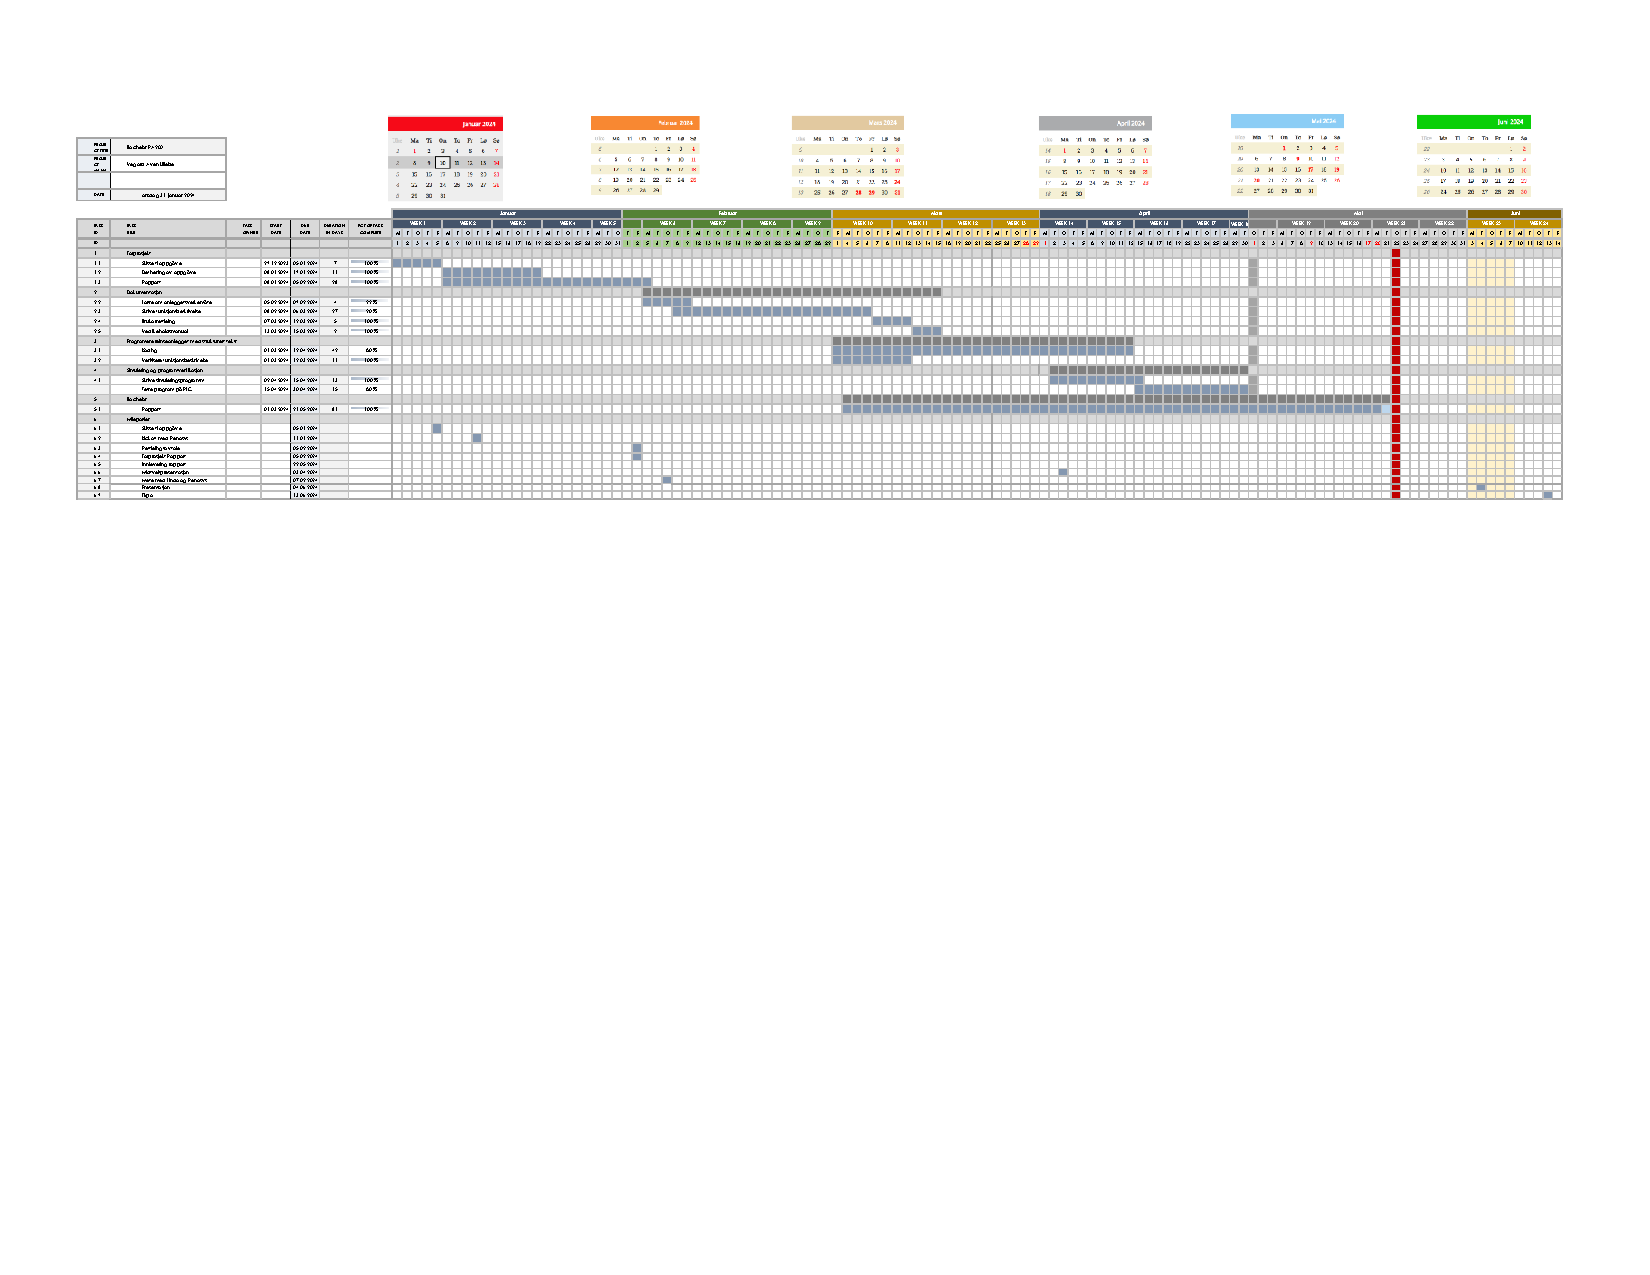
\includepdf[pages=1, angle=90,scale=0.8, pagecommand={\chapter{Gant}\thispagestyle{fancy}},fitpaper=true]{Vedlegg/Gant2.pdf}

% ------------ Nytt Kapittel

\thispagestyle{fancy}

% Sekvens Blokker 
% FB Pause
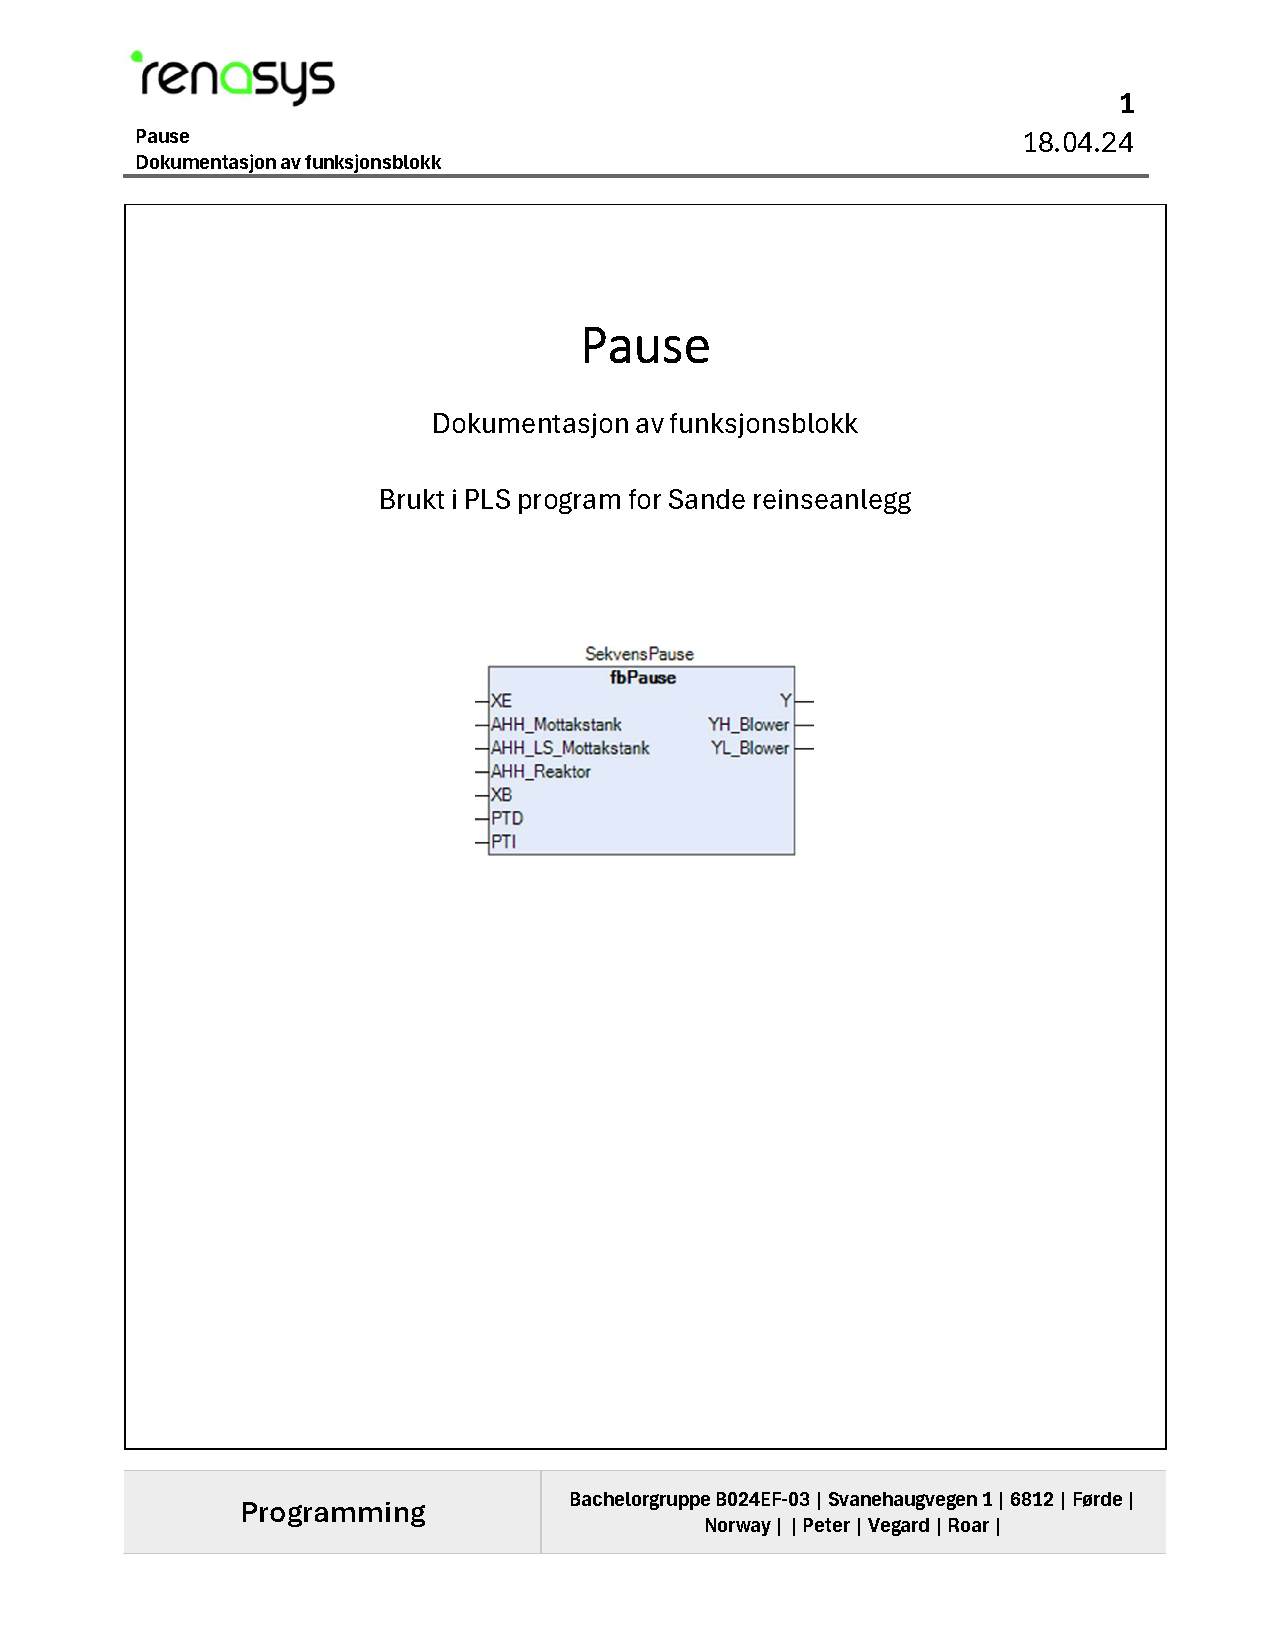
\includepdf[pages=1, scale=0.7, pagecommand={\chapter{Funksjons Blokker}, \section{FB Pause Sekvens}\thispagestyle{fancy}}, fitpaper=true ]{Vedlegg/Funksjons Blokker/fbPause.pdf}
\includepdf[pages=2-,scale=0.8, pagecommand={\thispagestyle{fancy}},fitpaper=true]{Vedlegg/Funksjons Blokker/fbPause.pdf}
% FB Innpumping
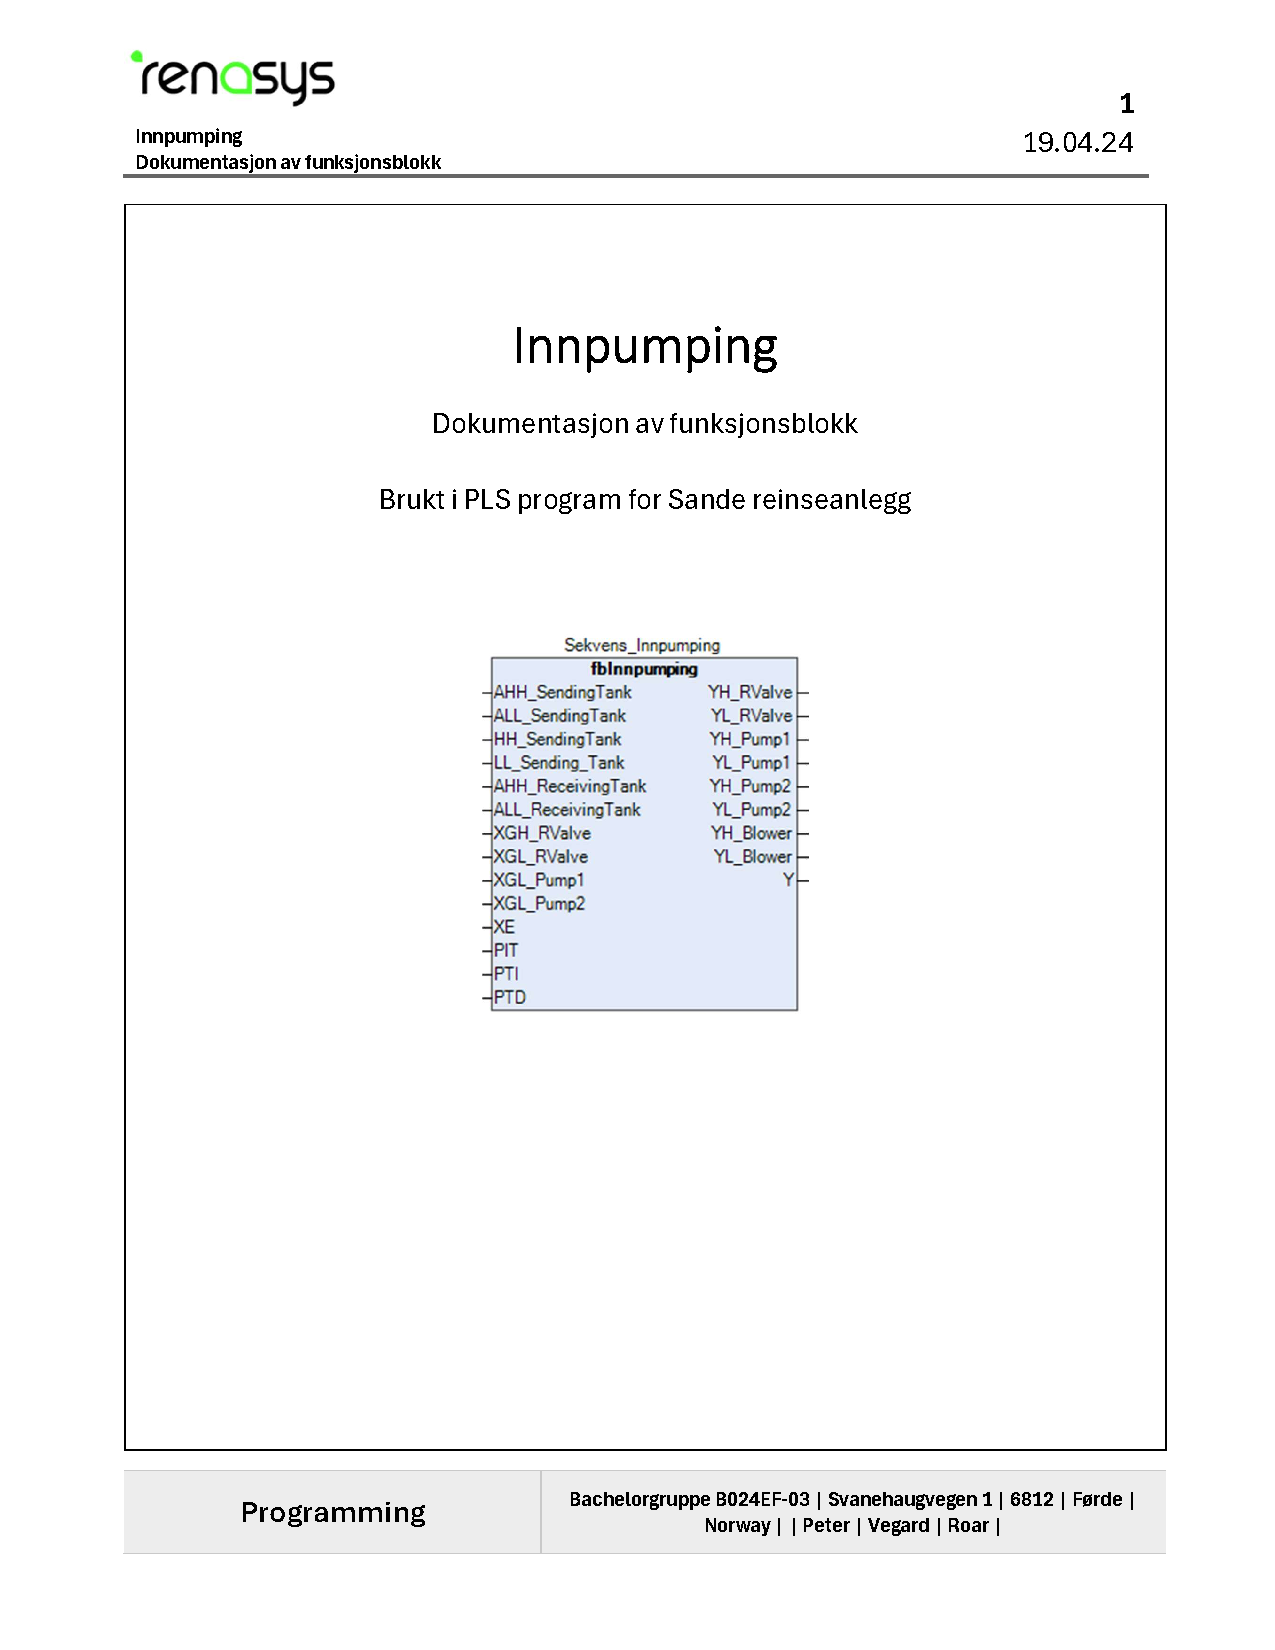
\includepdf[pages=1, scale=0.8, pagecommand={\section{FB Innpumpings Sekvens}\thispagestyle{fancy}}, fitpaper=true ]{Vedlegg/Funksjons Blokker/fbInnpumping.pdf}
\includepdf[pages=2-,scale=0.8, pagecommand={\thispagestyle{fancy}},fitpaper=true]{Vedlegg/Funksjons Blokker/fbInnpumping.pdf}
% FB Reaksjon
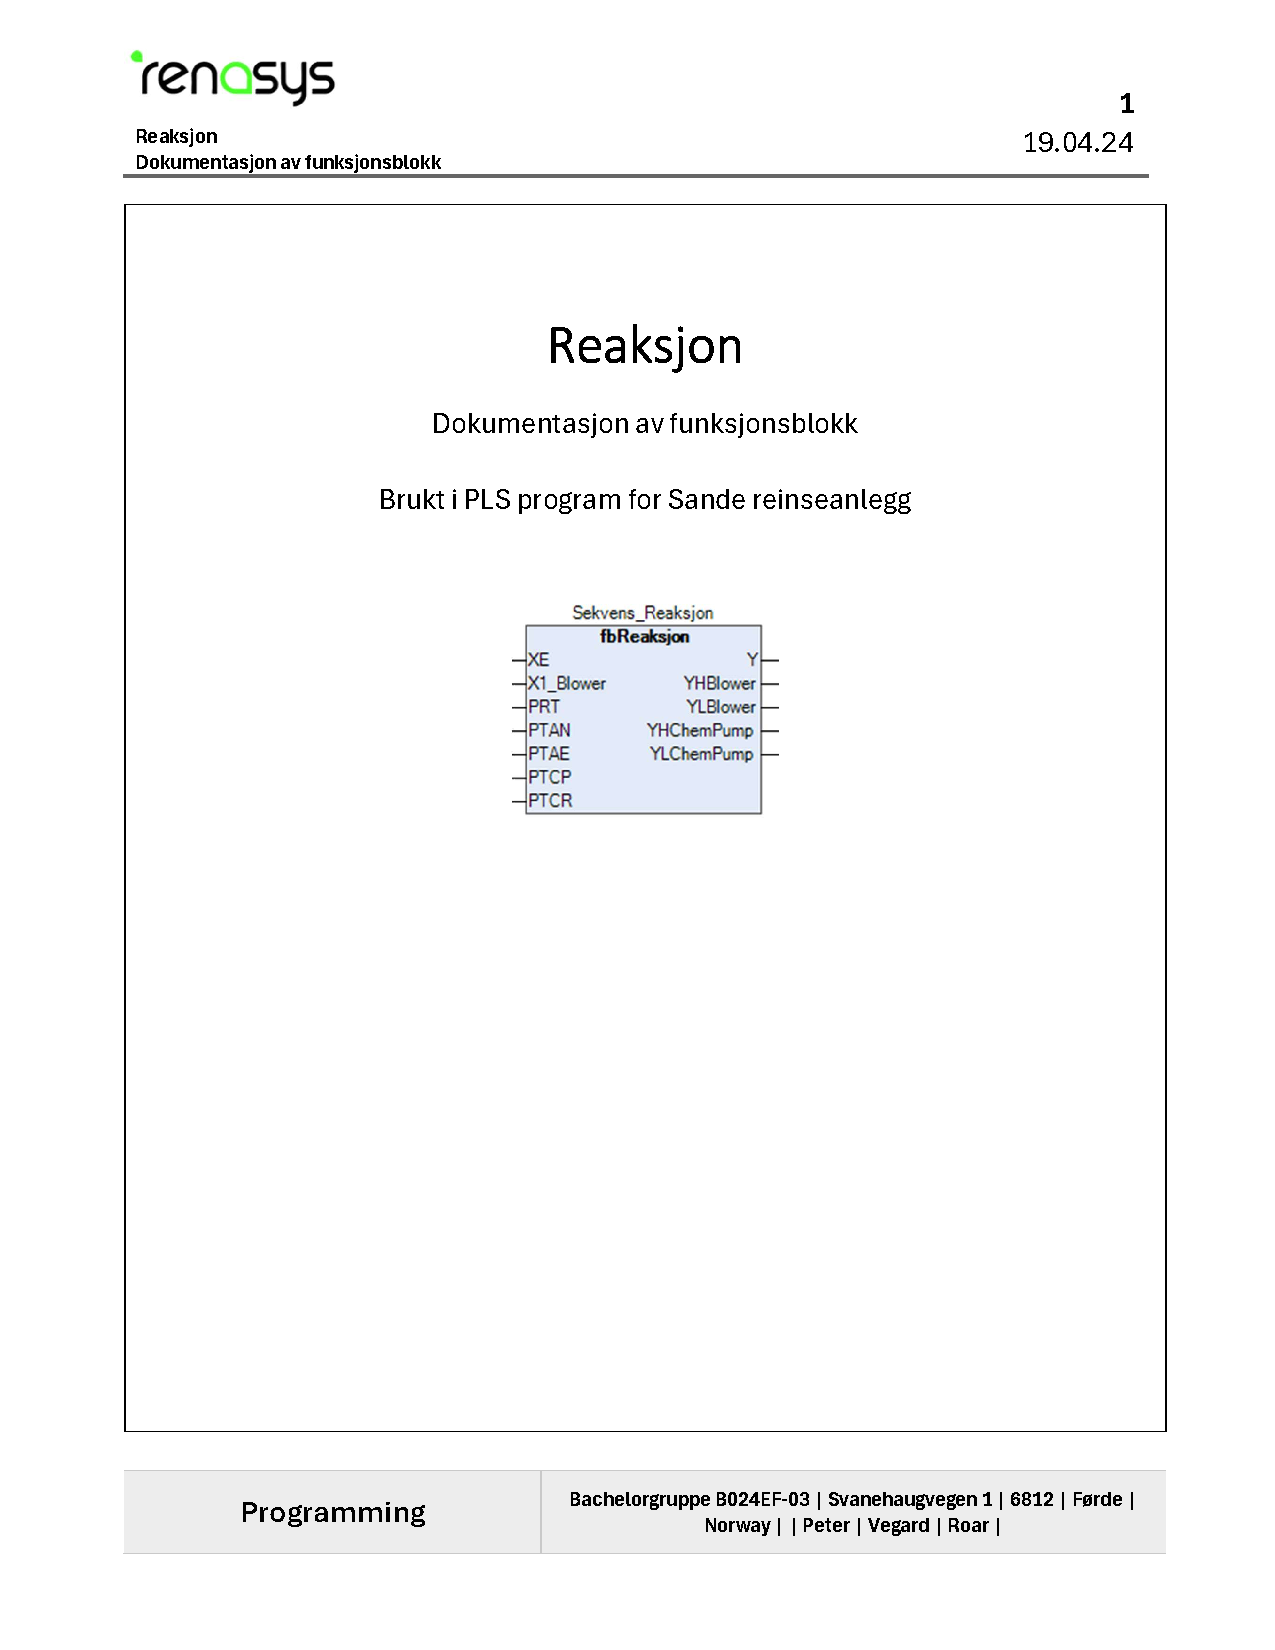
\includepdf[pages=1, scale=0.8, pagecommand={\section{FB Reaksjon Sekvens}\thispagestyle{fancy}}, fitpaper=true ]{Vedlegg/Funksjons Blokker/fbReaksjon Dokumentasjon.pdf}
\includepdf[pages=2-,scale=0.8, pagecommand={\thispagestyle{fancy}},fitpaper=true]{Vedlegg/Funksjons Blokker/fbReaksjon Dokumentasjon.pdf}
% FB Sedimentering
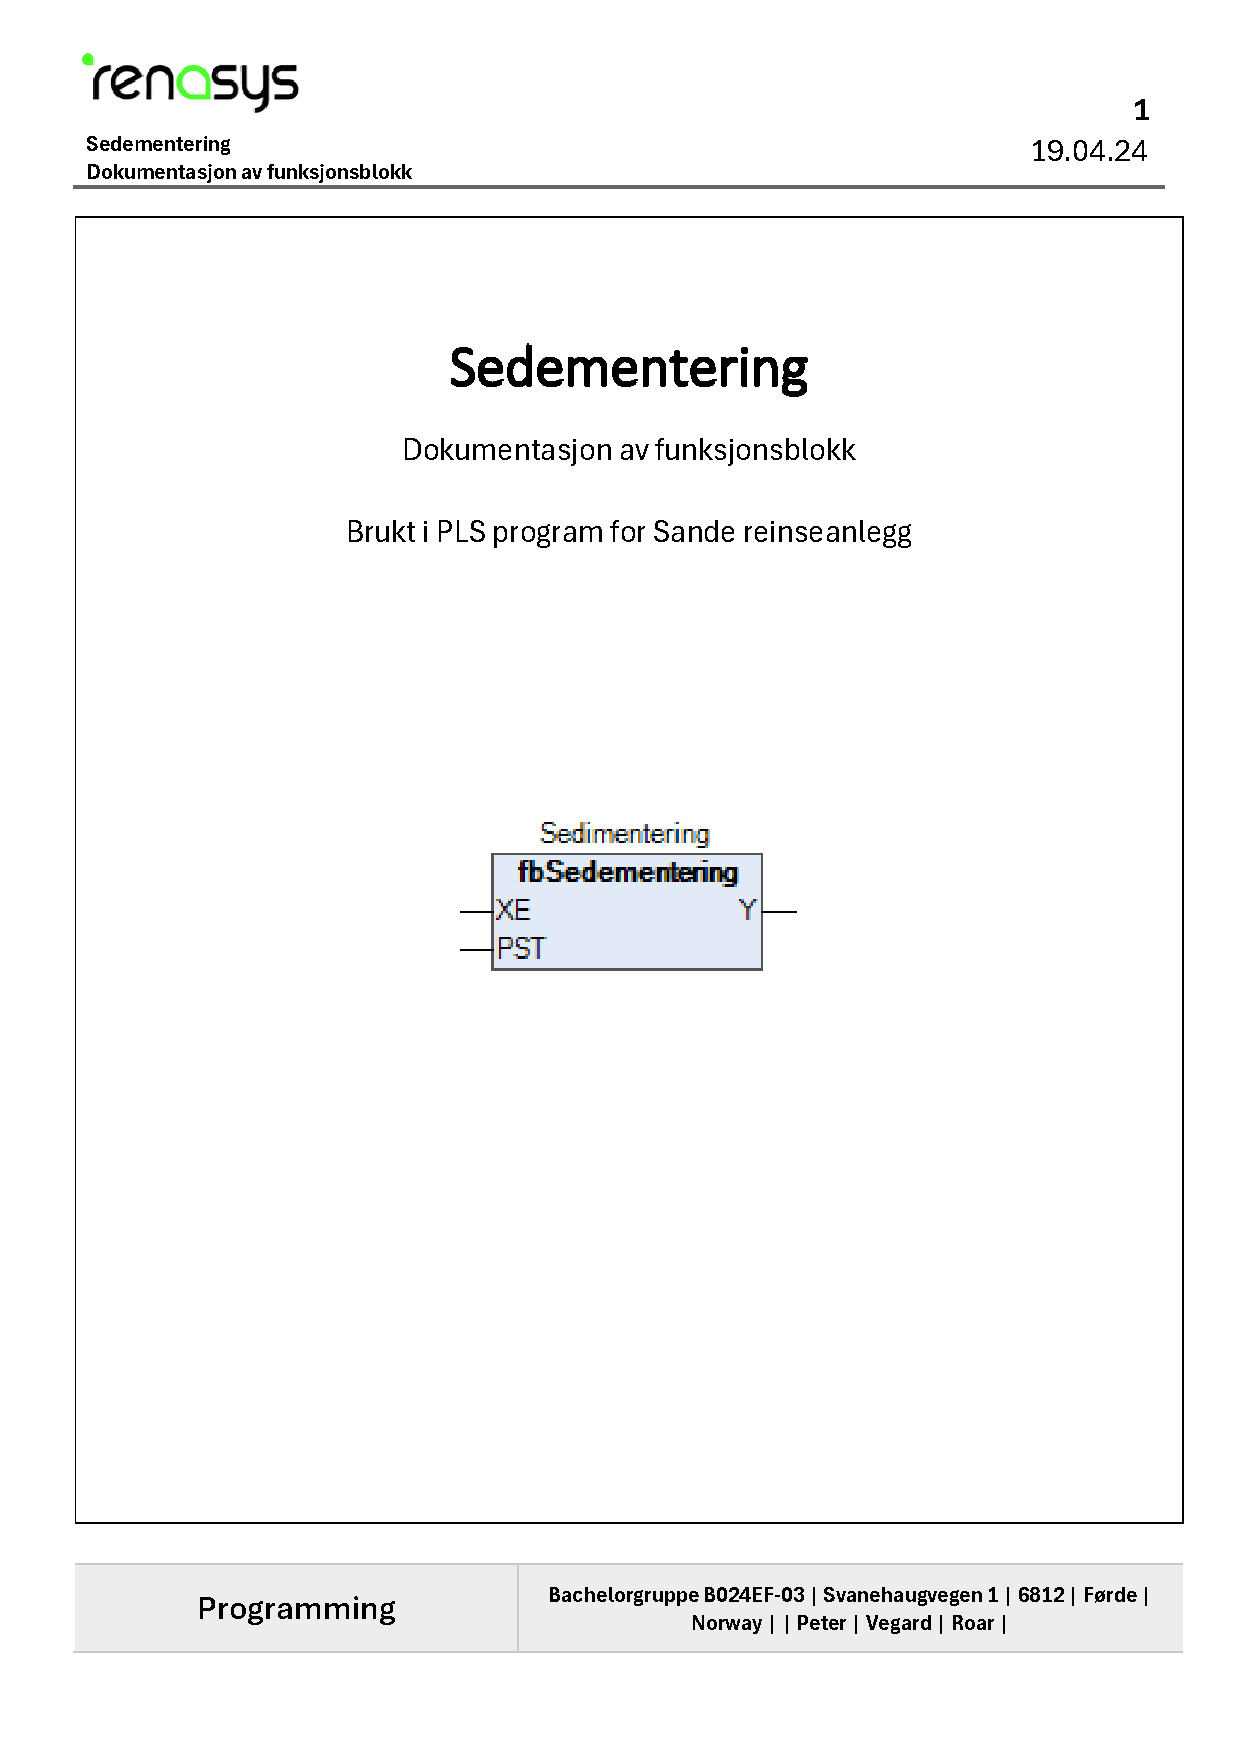
\includepdf[pages=1, scale=0.8, pagecommand={\section{FB Sedimentering Sekvens}\thispagestyle{fancy}}, fitpaper=true ]{Vedlegg/Funksjons Blokker/fbSedementering Dokumentasjon.pdf}
\includepdf[pages=2-,scale=0.8, pagecommand={\thispagestyle{fancy}},fitpaper=true]{Vedlegg/Funksjons Blokker/fbSedementering Dokumentasjon.pdf}
% FB Uttapping
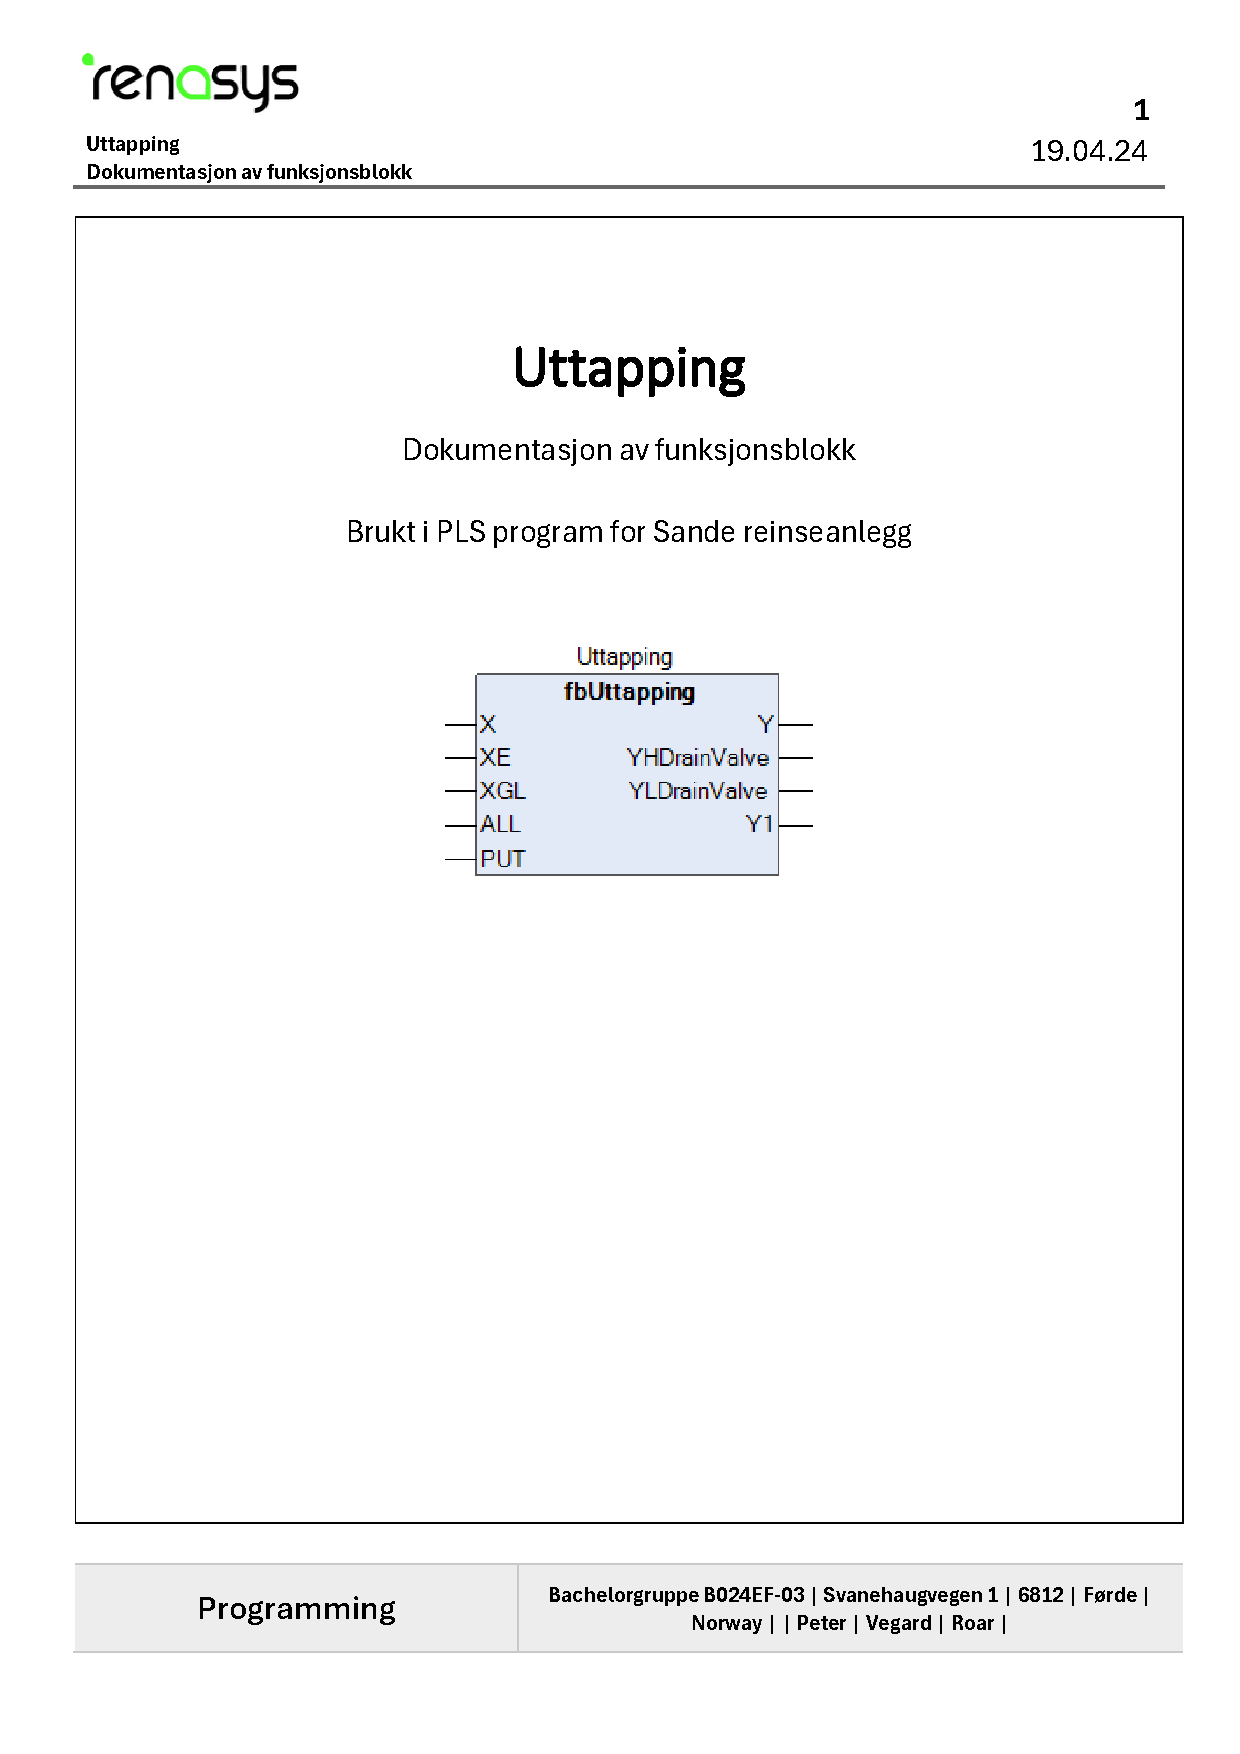
\includepdf[pages=1, scale=0.8, pagecommand={\section{FB Uttapping Sekvens}\thispagestyle{fancy}}, fitpaper=true ]{Vedlegg/Funksjons Blokker/fbUttaping Dokumentasjon.pdf}
\includepdf[pages=2-,scale=0.8, pagecommand={\thispagestyle{fancy}},fitpaper=true]{Vedlegg/Funksjons Blokker/fbUttaping Dokumentasjon.pdf}
% FB Slammuttak
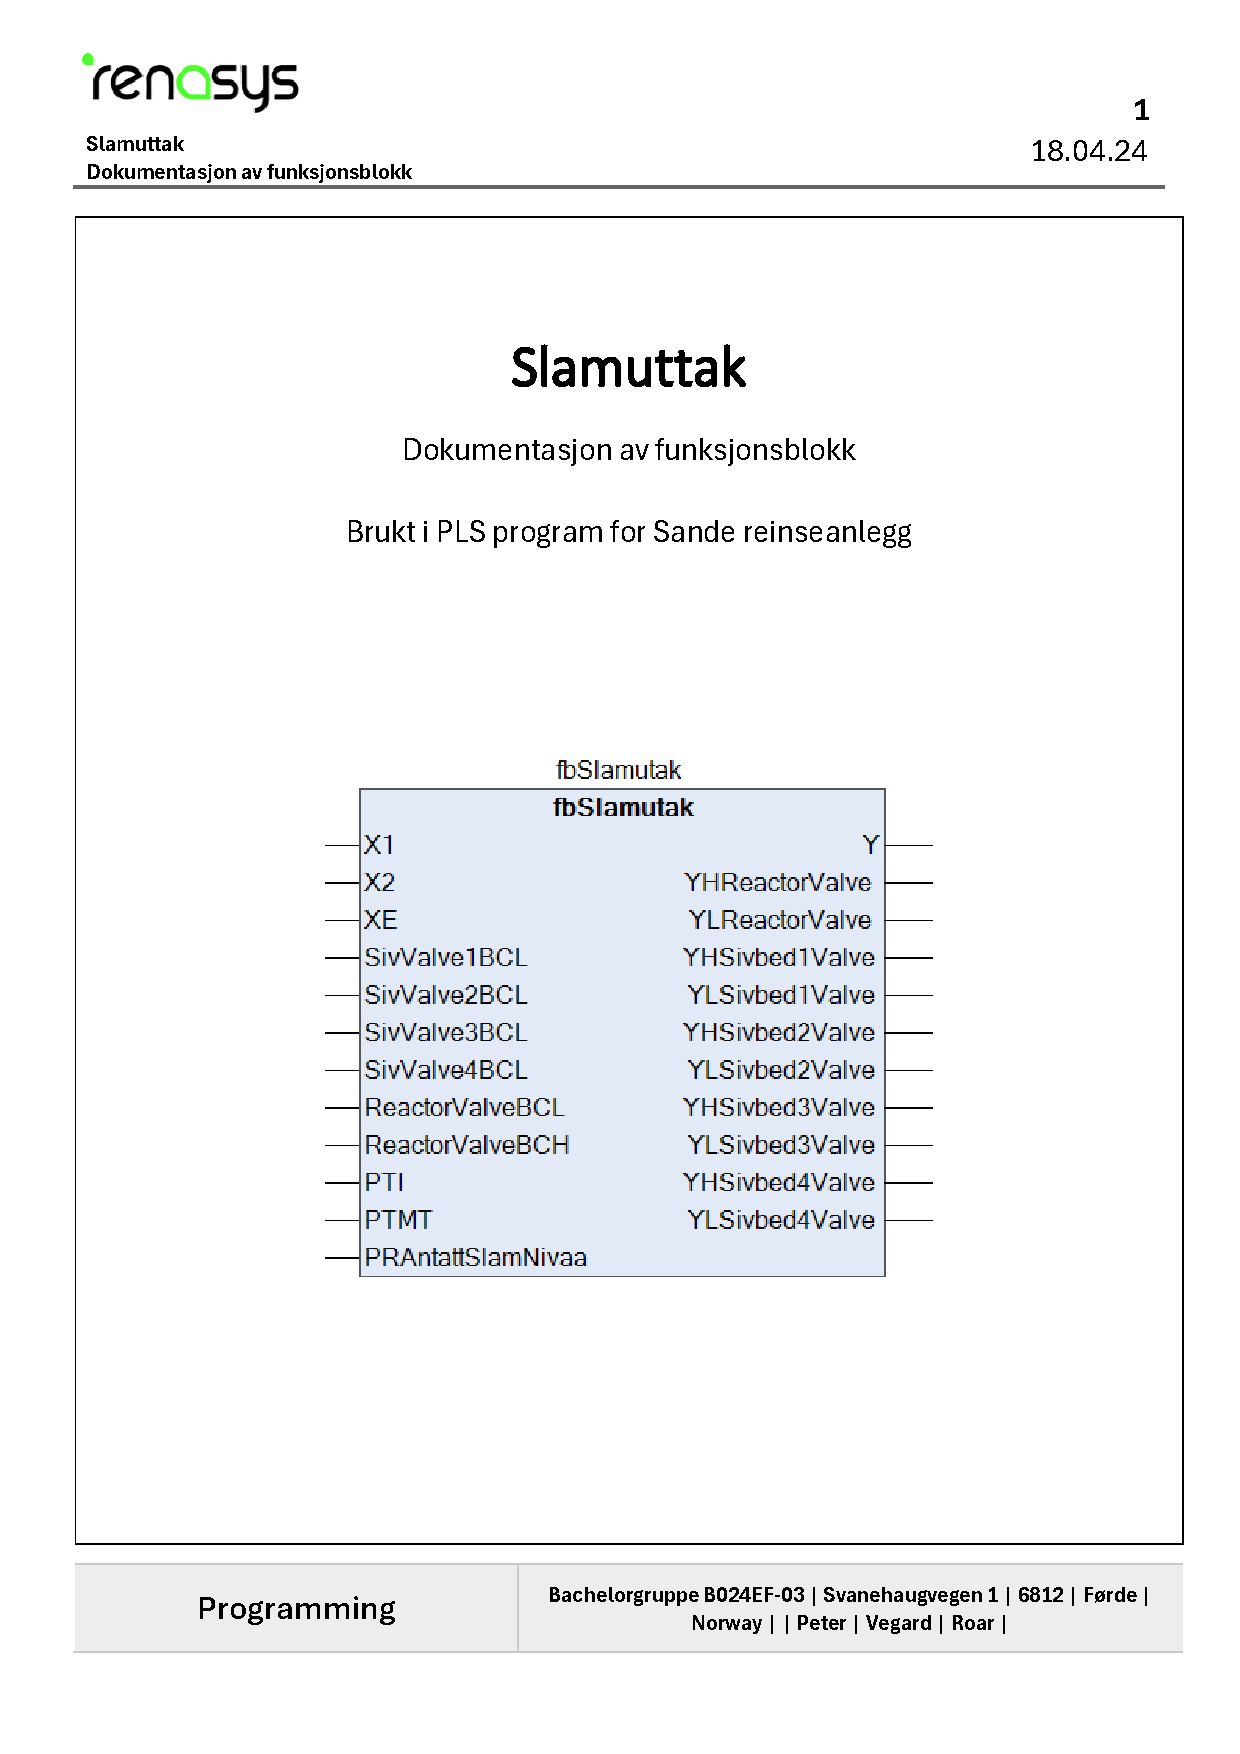
\includepdf[pages=1, scale=0.8, pagecommand={\section{FB Slammuttak}\thispagestyle{fancy}}, fitpaper=true ]{Vedlegg/Funksjons Blokker/fbSlamuttak Dokumentasjon.pdf}
\includepdf[pages=2-,scale=0.8, pagecommand={\thispagestyle{fancy}},fitpaper=true]{Vedlegg/Funksjons Blokker/fbSlamuttak Dokumentasjon.pdf}
% 
% Analog Alarm
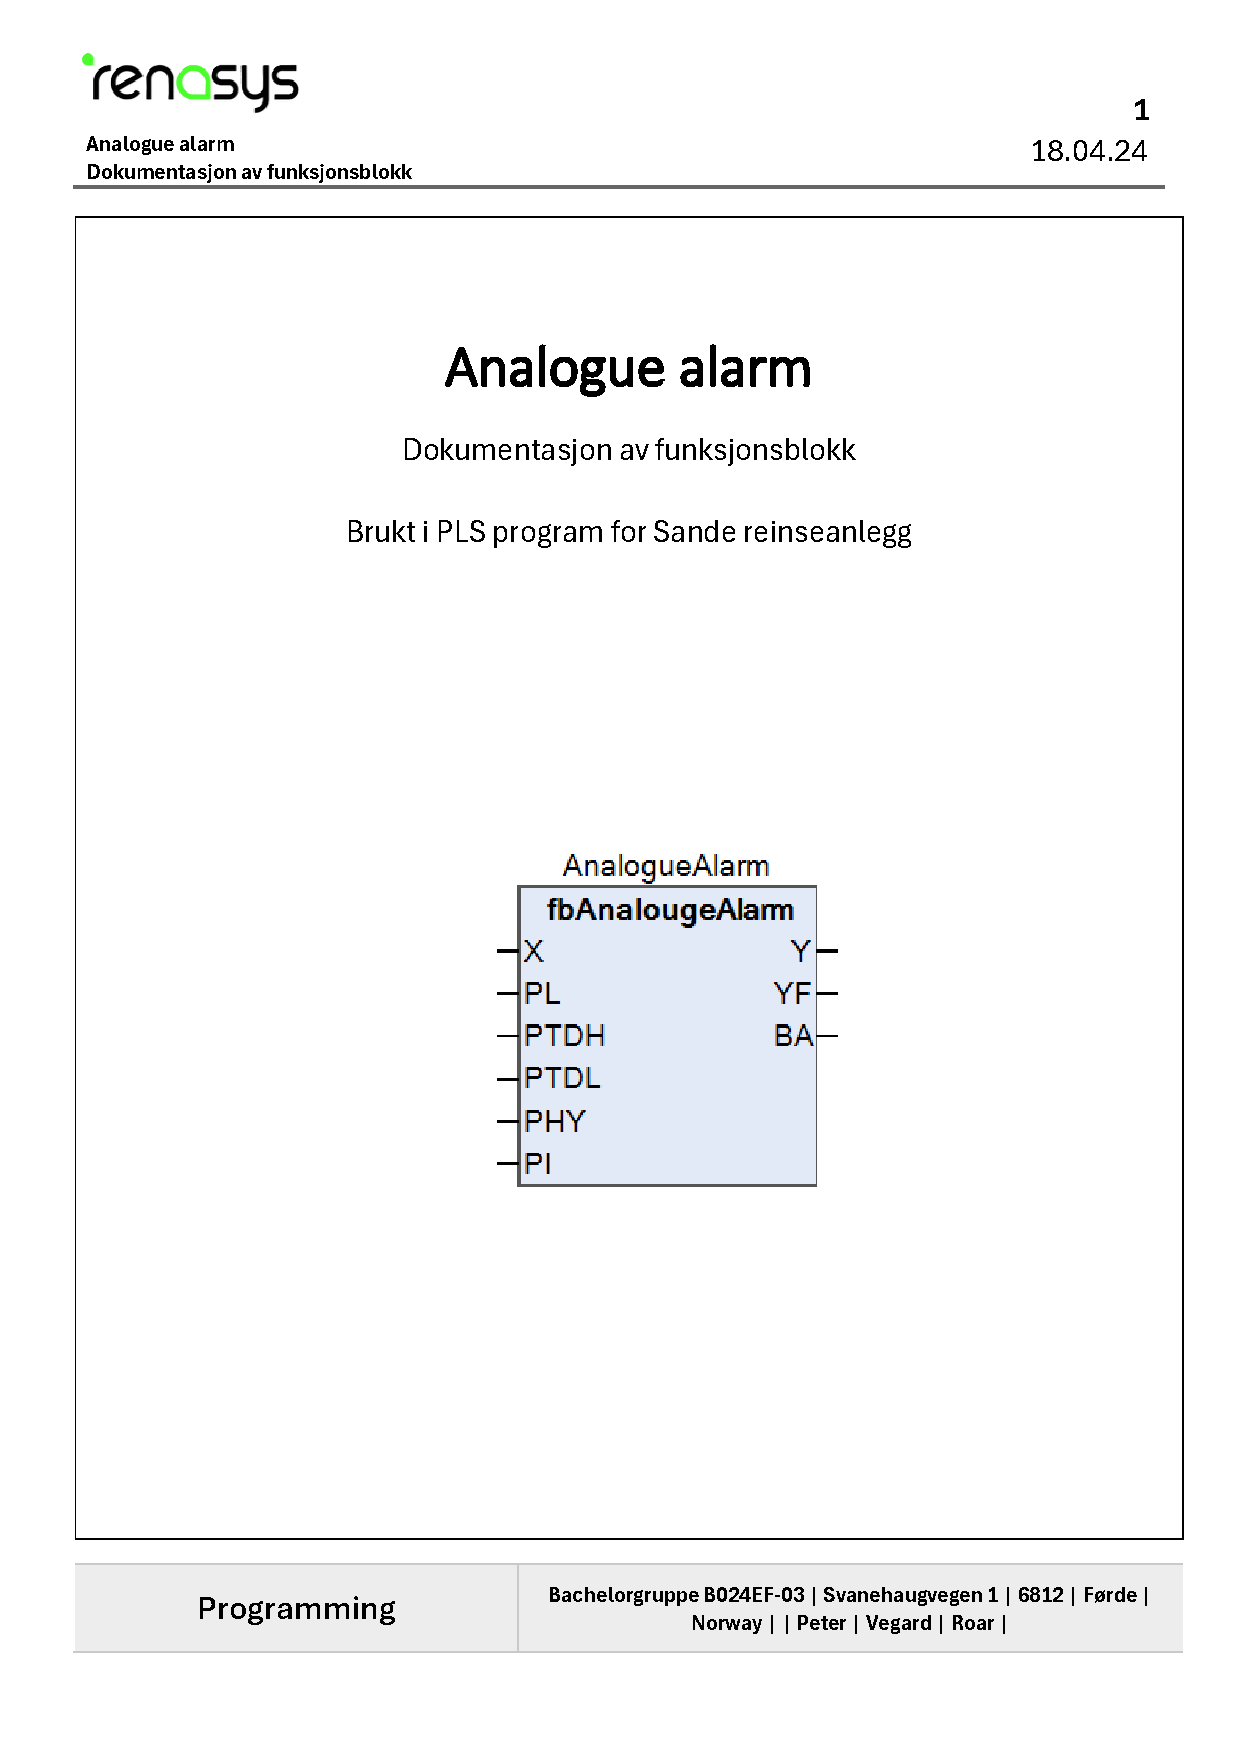
\includepdf[pages=1, scale=0.8, pagecommand={\section{FB Analog alarm}\thispagestyle{fancy}}, fitpaper=true ]{Vedlegg/Funksjons Blokker/fbAnalogueAlarm Dokumentasjon.pdf}
\includepdf[pages=2-,scale=0.8, pagecommand={\thispagestyle{fancy}},fitpaper=true]{Vedlegg/Funksjons Blokker/fbAnalogueAlarm Dokumentasjon.pdf}
% Digital Alarm
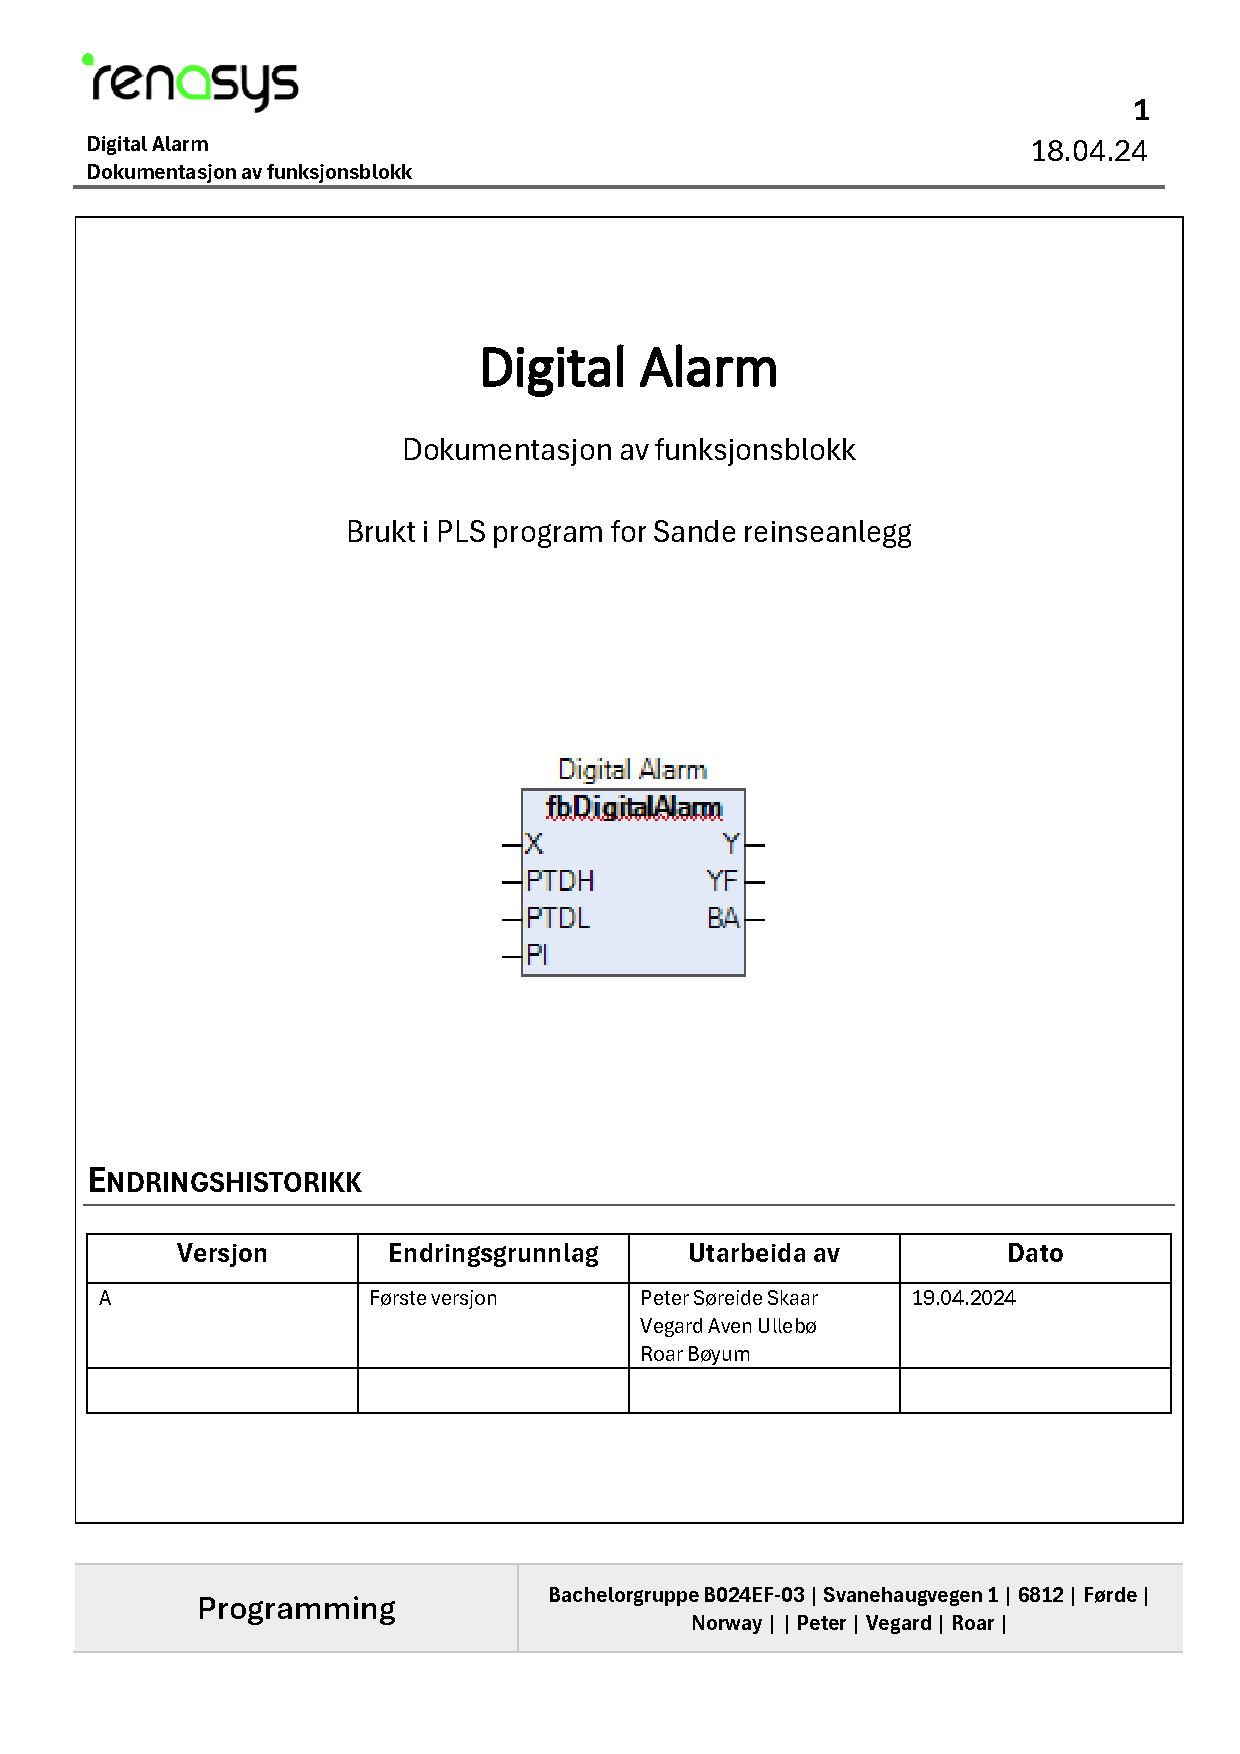
\includepdf[pages=1, scale=0.8, pagecommand={\section{FB Digital alarm}\thispagestyle{fancy}}, fitpaper=true ]{Vedlegg/Funksjons Blokker/fbDigitalAlarm.pdf}
\includepdf[pages=2-,scale=0.8, pagecommand={\thispagestyle{fancy}},fitpaper=true]{Vedlegg/Funksjons Blokker/fbDigitalAlarm.pdf}
% Calculations
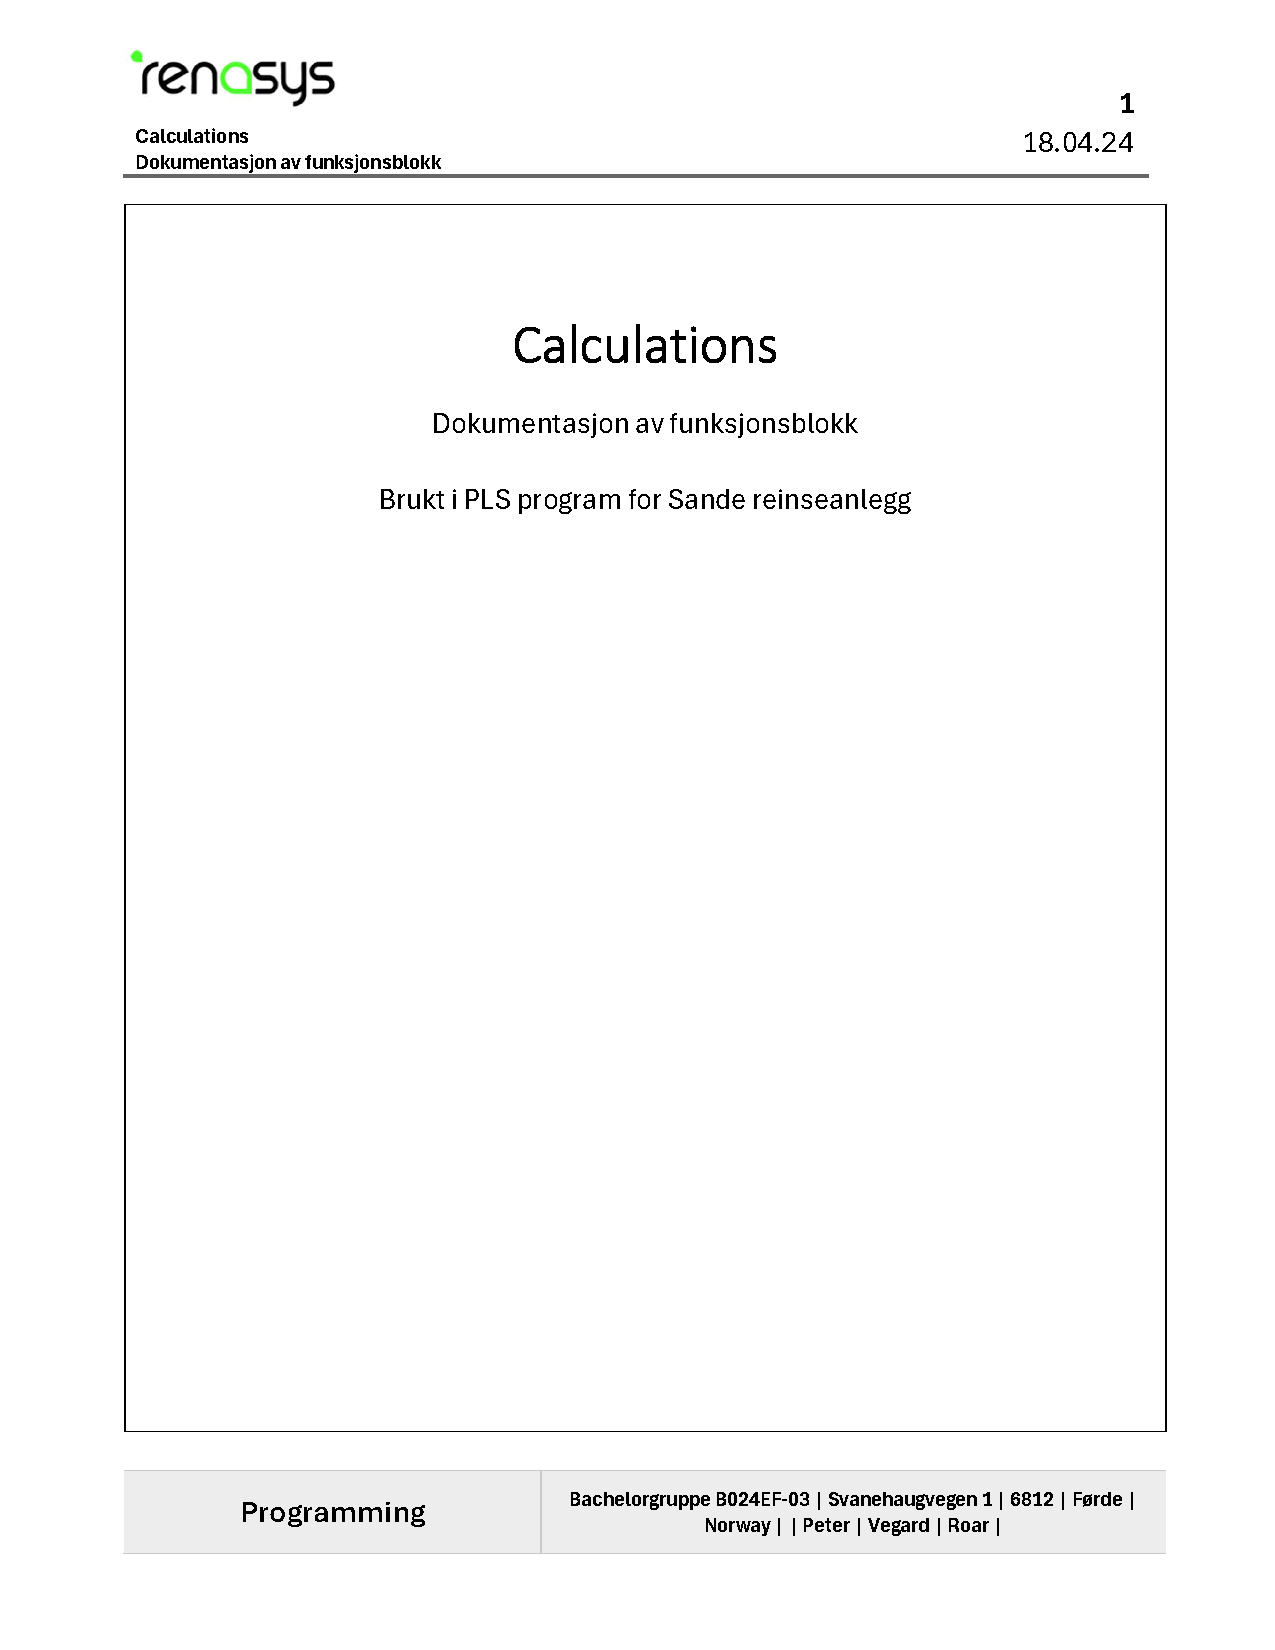
\includepdf[pages=1, scale=0.8, pagecommand={\section{FB Kalkuleringer}\thispagestyle{fancy}}, fitpaper=true ]{Vedlegg/Funksjons Blokker/fbCalculations.pdf}
\includepdf[pages=2-,scale=0.8, pagecommand={\thispagestyle{fancy}},fitpaper=true]{Vedlegg/Funksjons Blokker/fbCalculations.pdf}
% Data Processing
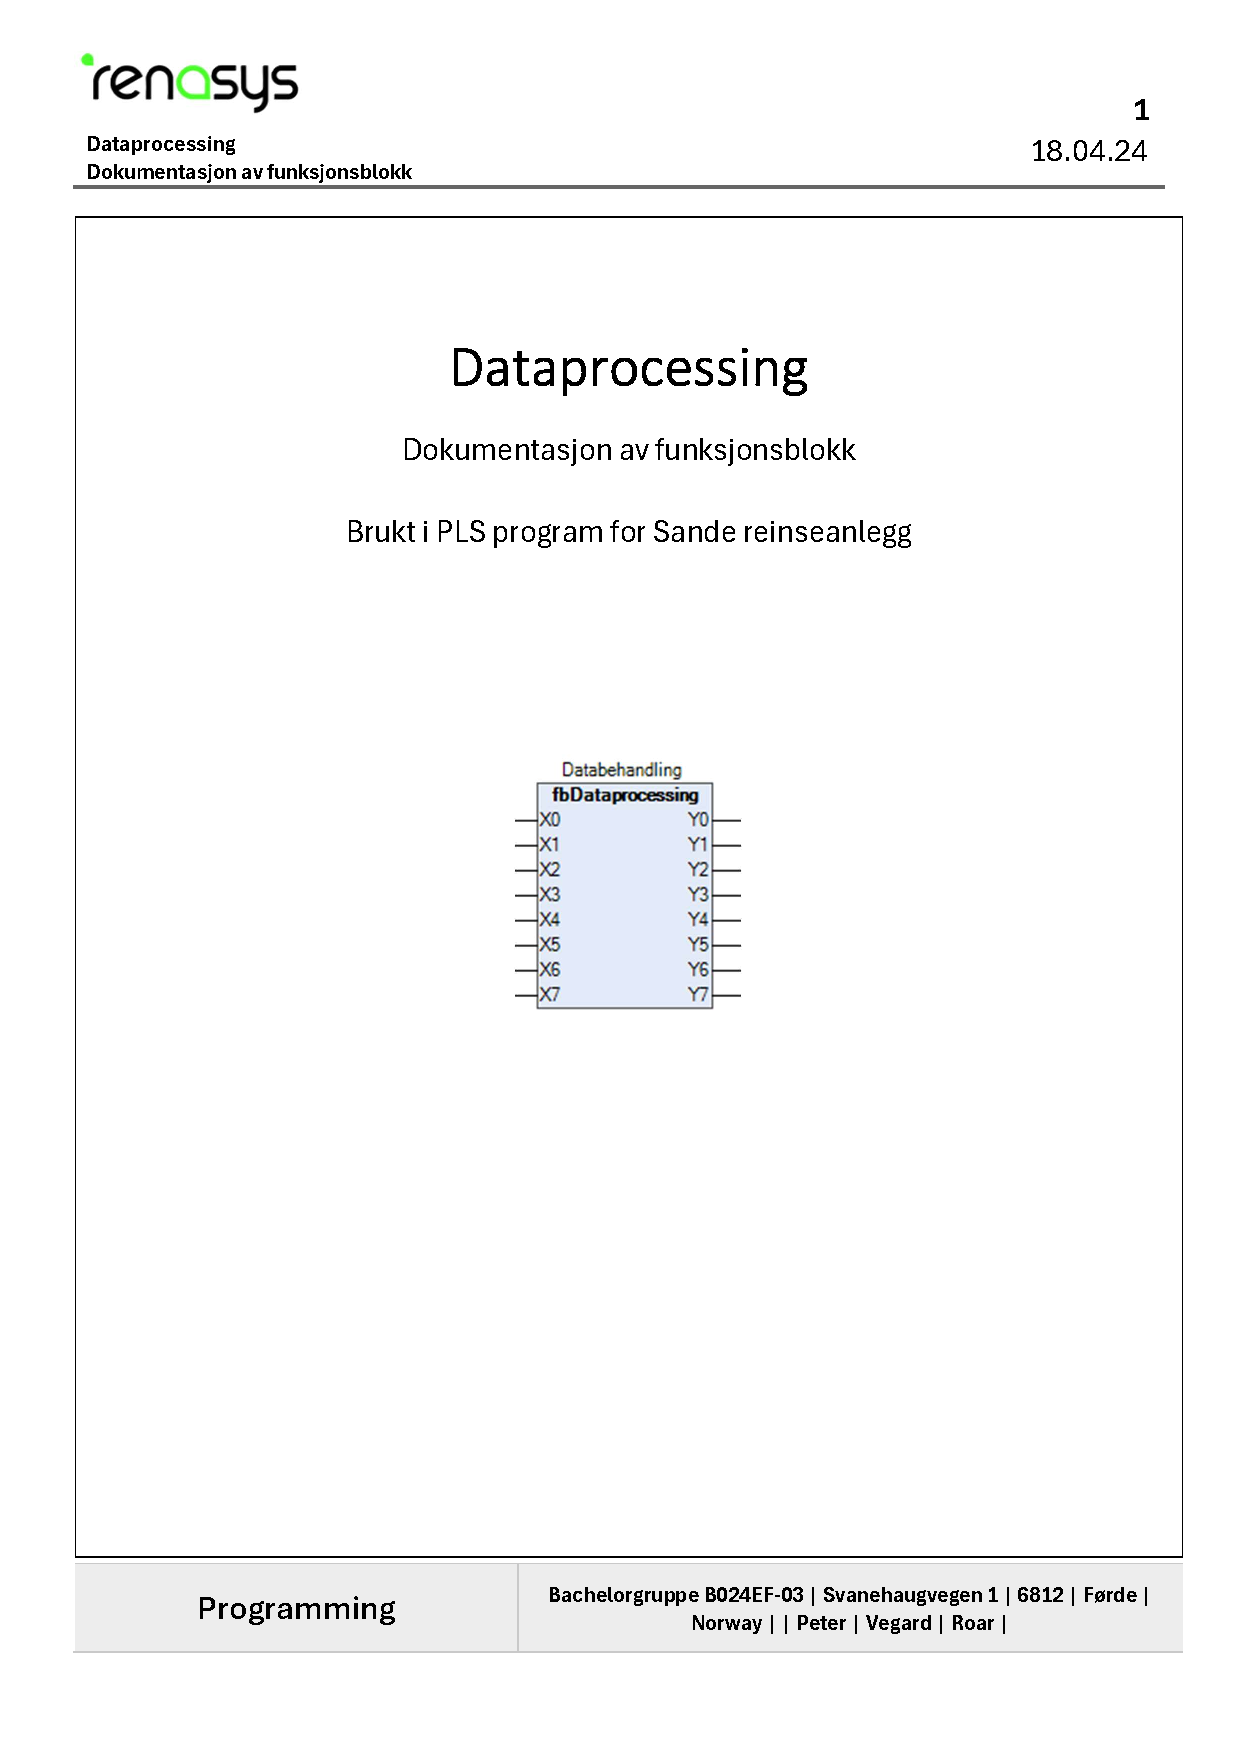
\includepdf[pages=1, scale=0.8, pagecommand={\section{FB Data Prossesering}\thispagestyle{fancy}}, fitpaper=true ]{Vedlegg/Funksjons Blokker/fbDataProcessing.pdf}
\includepdf[pages=2-,scale=0.8, pagecommand={\thispagestyle{fancy}},fitpaper=true]{Vedlegg/Funksjons Blokker/fbDataProcessing.pdf}
% Høgbelastningsmodus
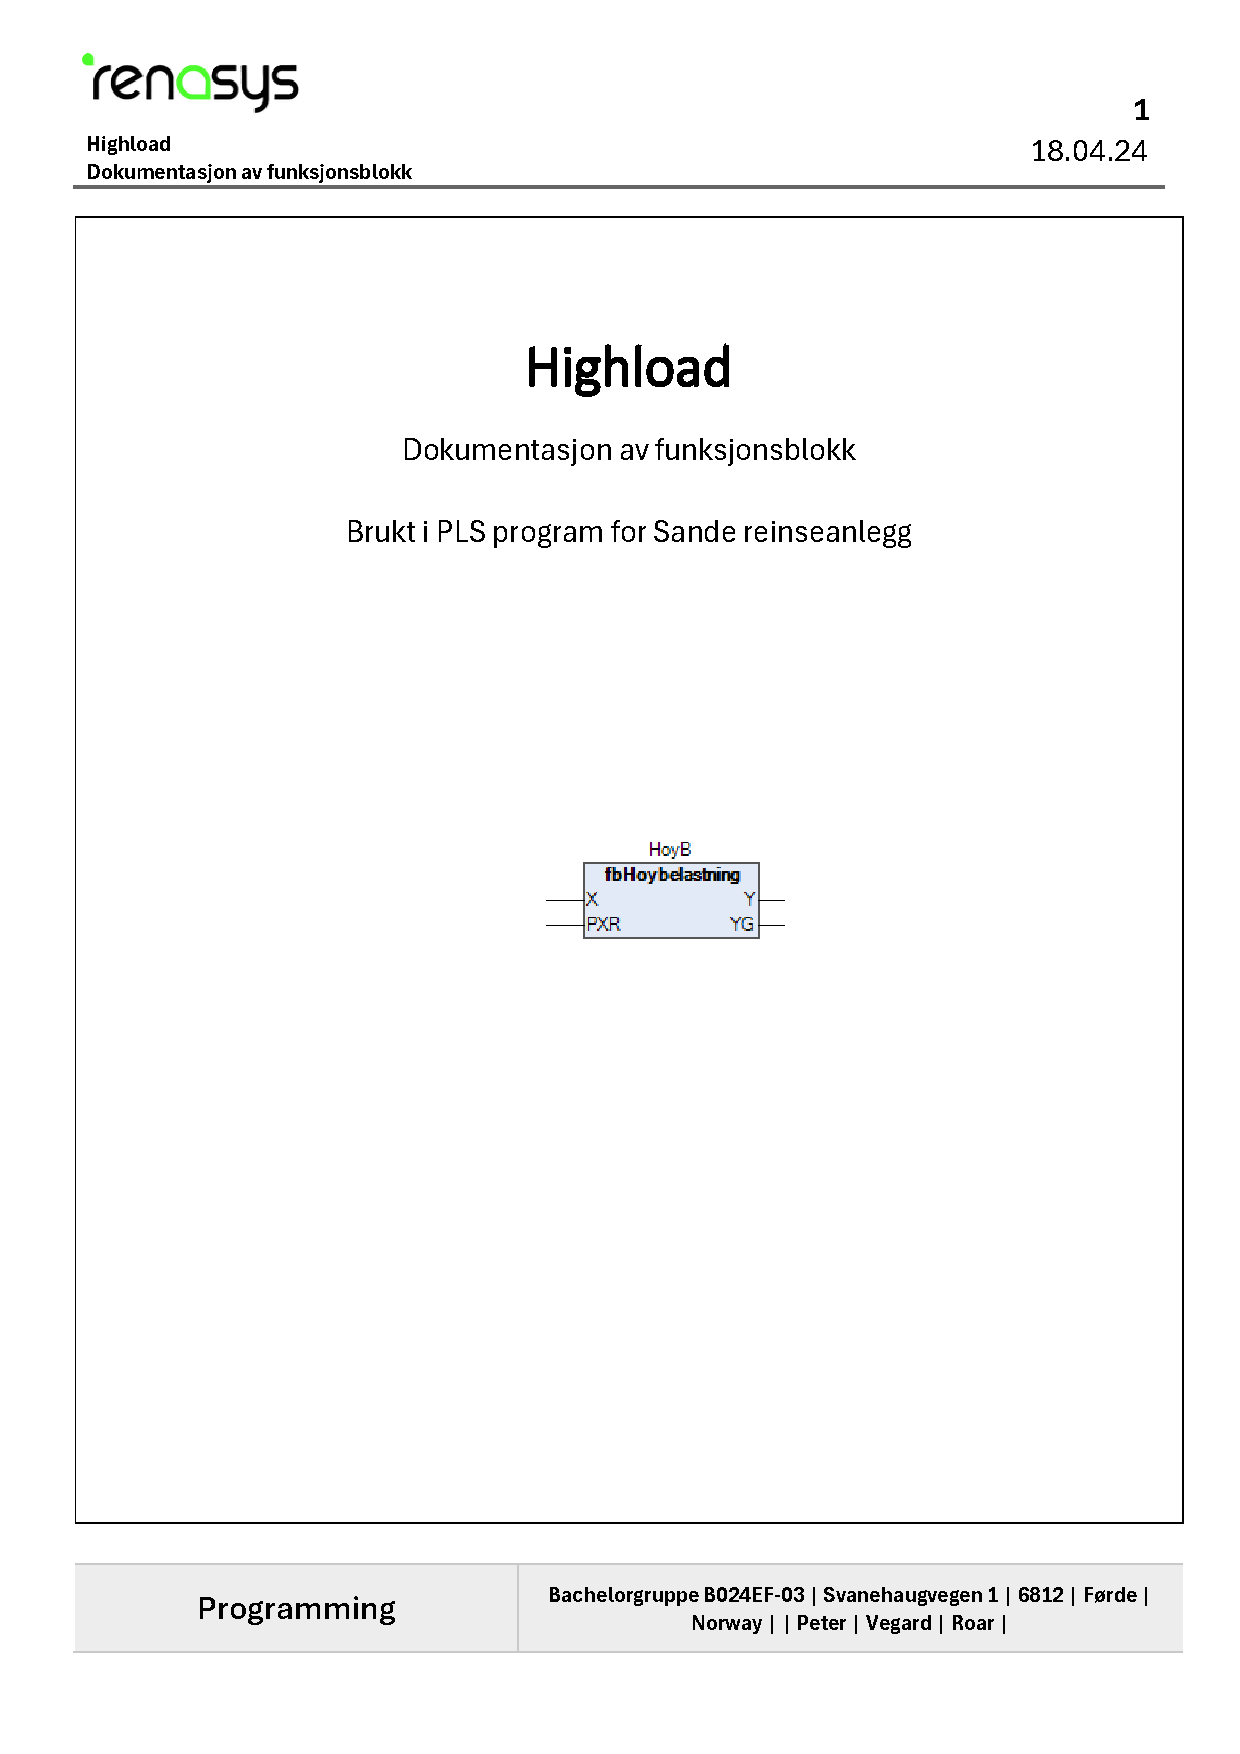
\includepdf[pages=1, scale=0.8, pagecommand={\section{FB High Load}\thispagestyle{fancy}}, fitpaper=true ]{Vedlegg/Funksjons Blokker/fbHighLoad.pdf}
\includepdf[pages=2-,scale=0.8, pagecommand={\thispagestyle{fancy}},fitpaper=true]{Vedlegg/Funksjons Blokker/fbHighLoad.pdf}
% Processed Water
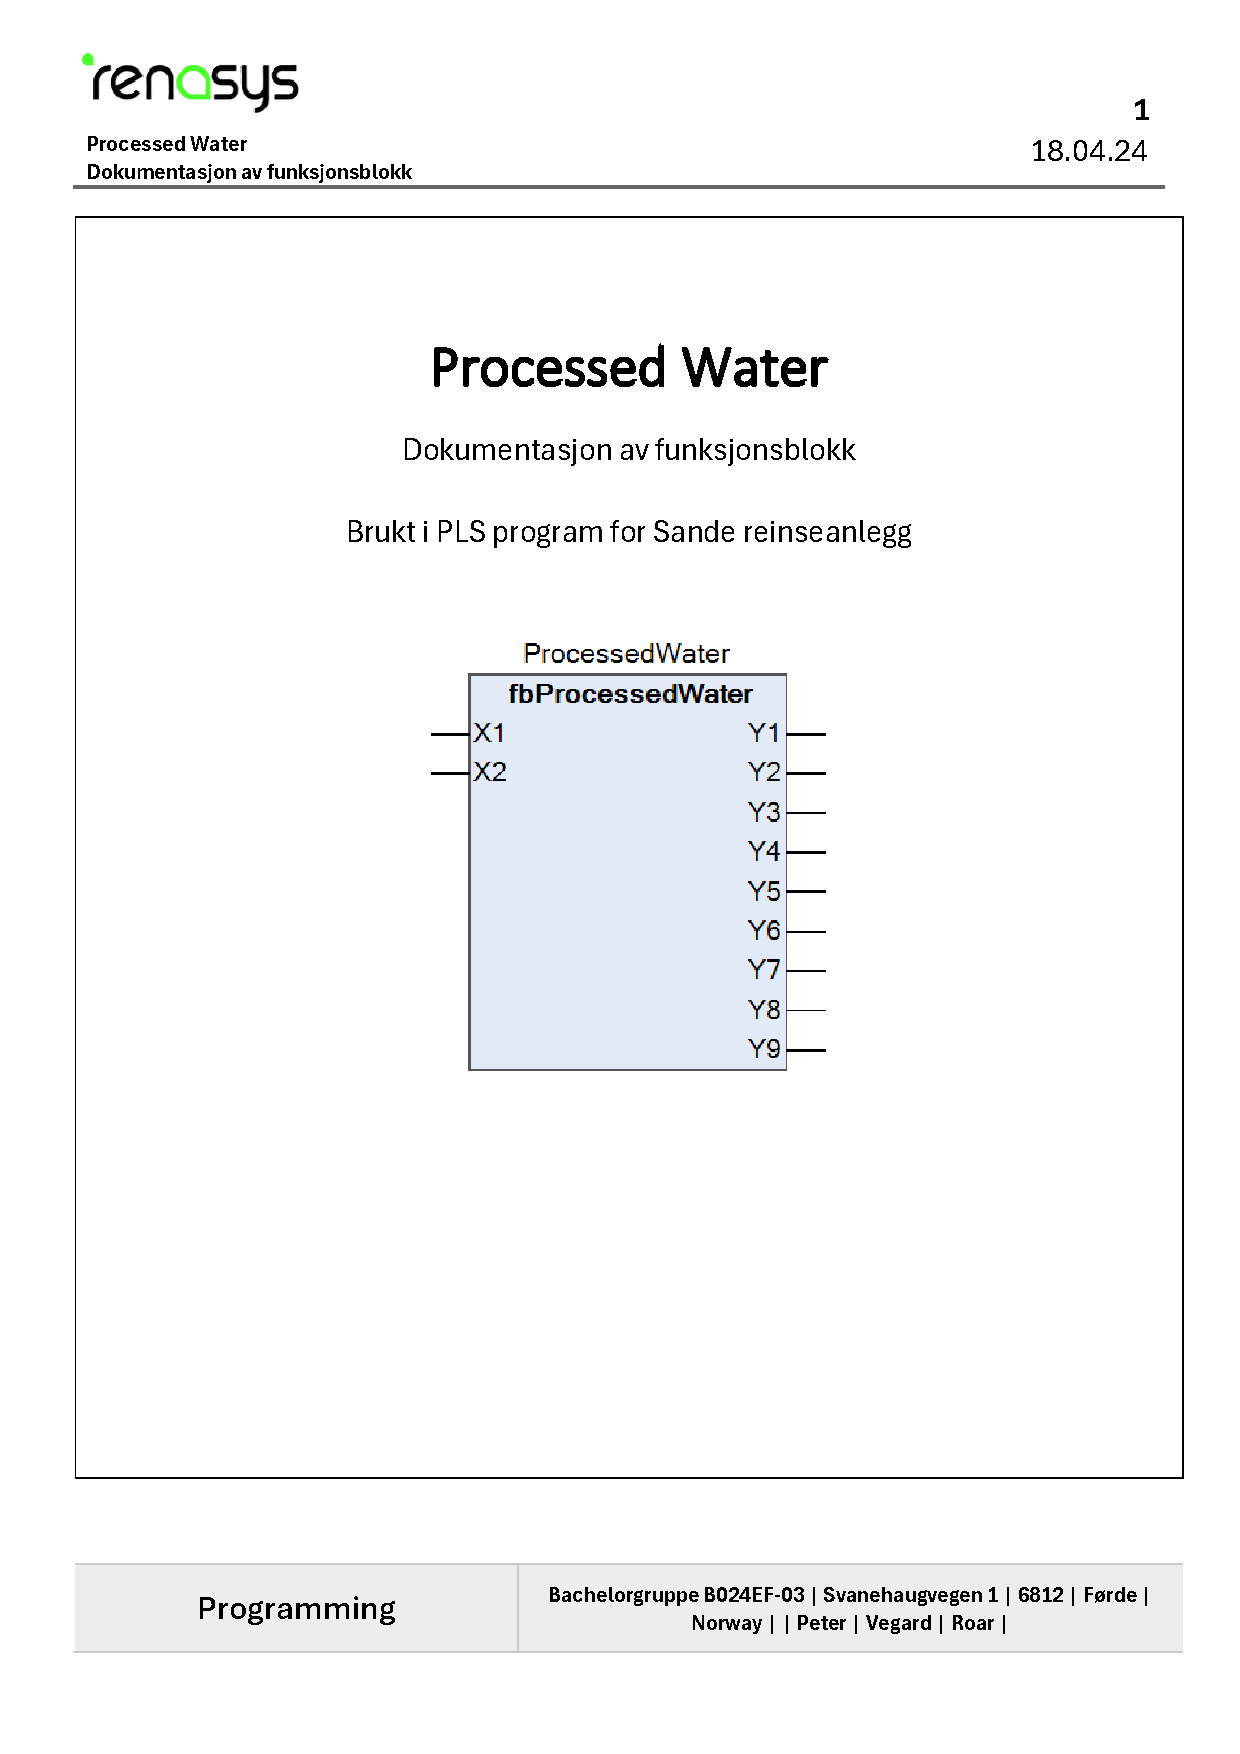
\includepdf[pages=1, scale=0.8, pagecommand={\section{FB Processed Water}\thispagestyle{fancy}}, fitpaper=true ]{Vedlegg/Funksjons Blokker/fbProcessedWater Dokumentasjon.pdf}
\includepdf[pages=2-,scale=0.8, pagecommand={\thispagestyle{fancy}},fitpaper=true]{Vedlegg/Funksjons Blokker/fbProcessedWater Dokumentasjon.pdf}
% fbPumpInterlock
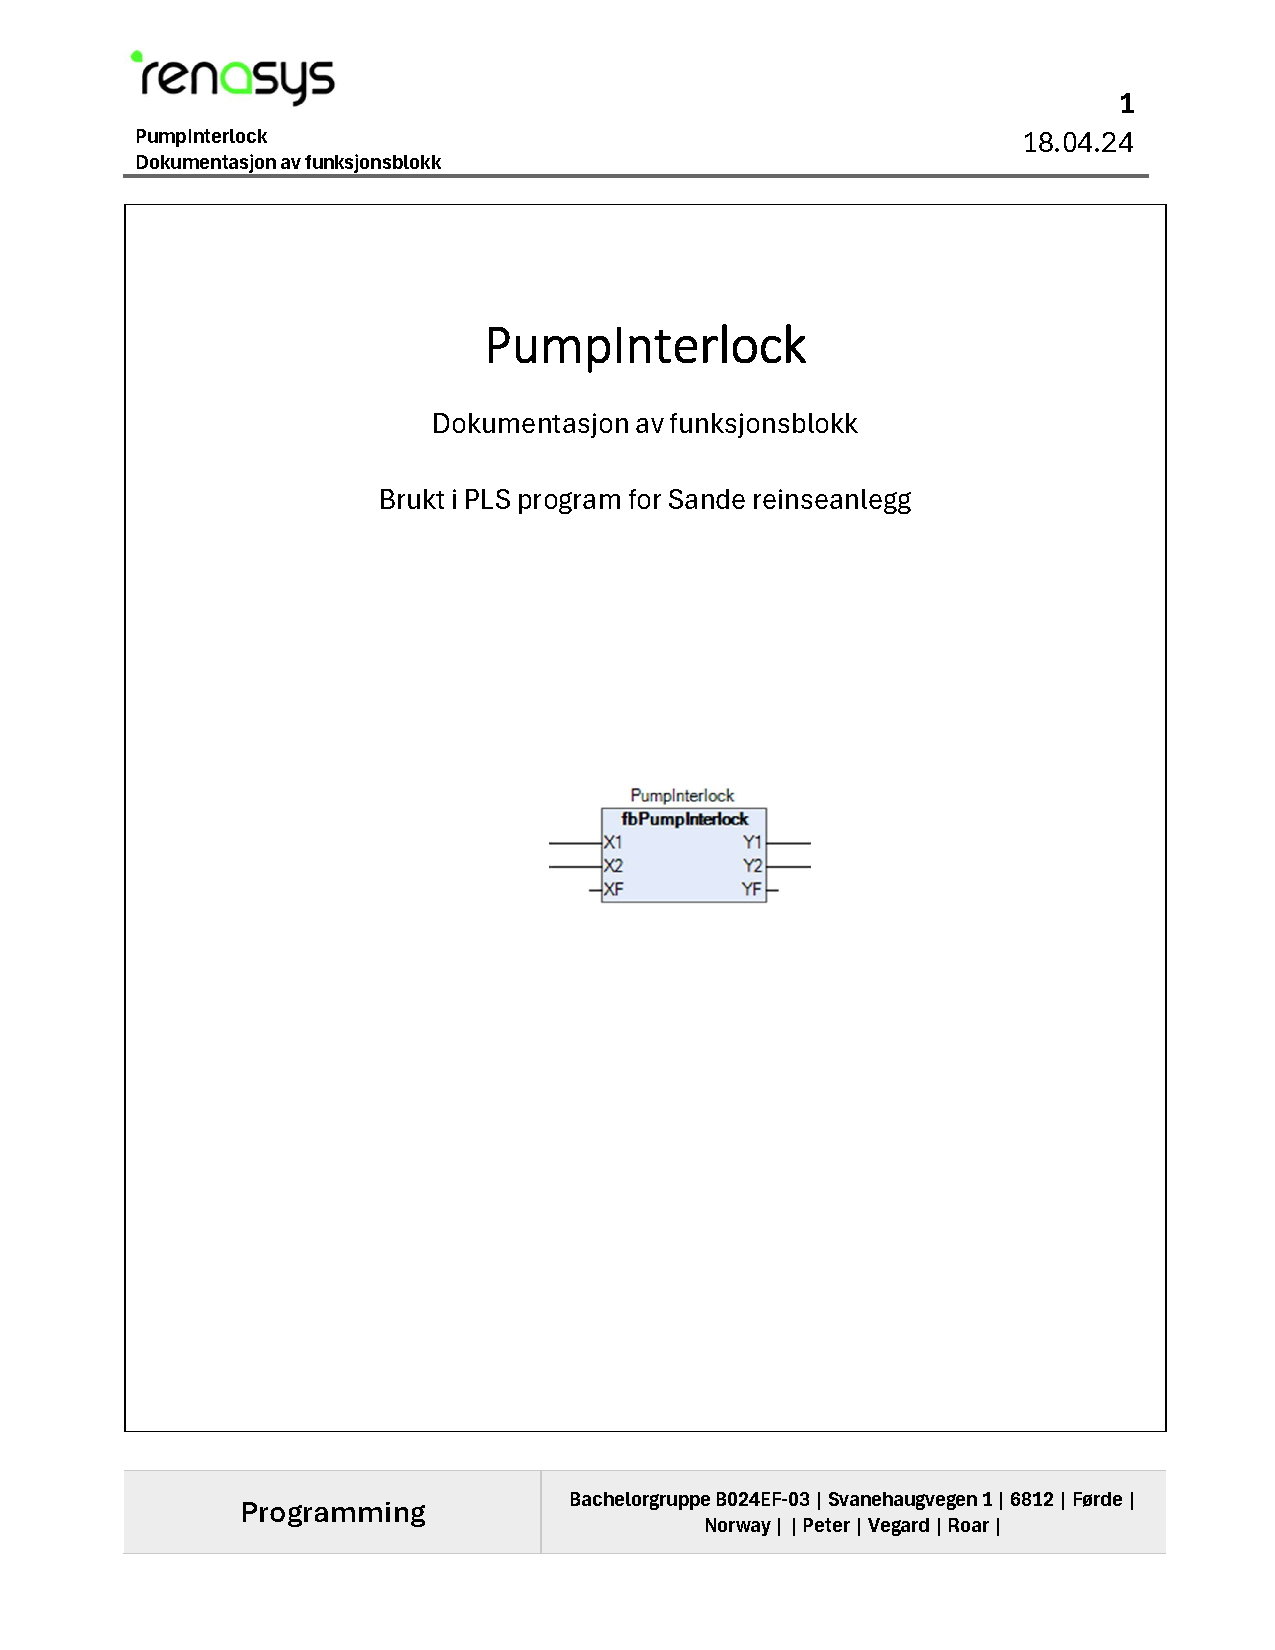
\includepdf[pages=1, scale=0.8, pagecommand={\section{FB Pump Interlock}\thispagestyle{fancy}}, fitpaper=true ]{Vedlegg/Funksjons Blokker/fbPumpInterlock.pdf}
\includepdf[pages=2-,scale=0.8, pagecommand={\thispagestyle{fancy}},fitpaper=true]{Vedlegg/Funksjons Blokker/fbPumpInterlock.pdf}
% Sivbed Rotation
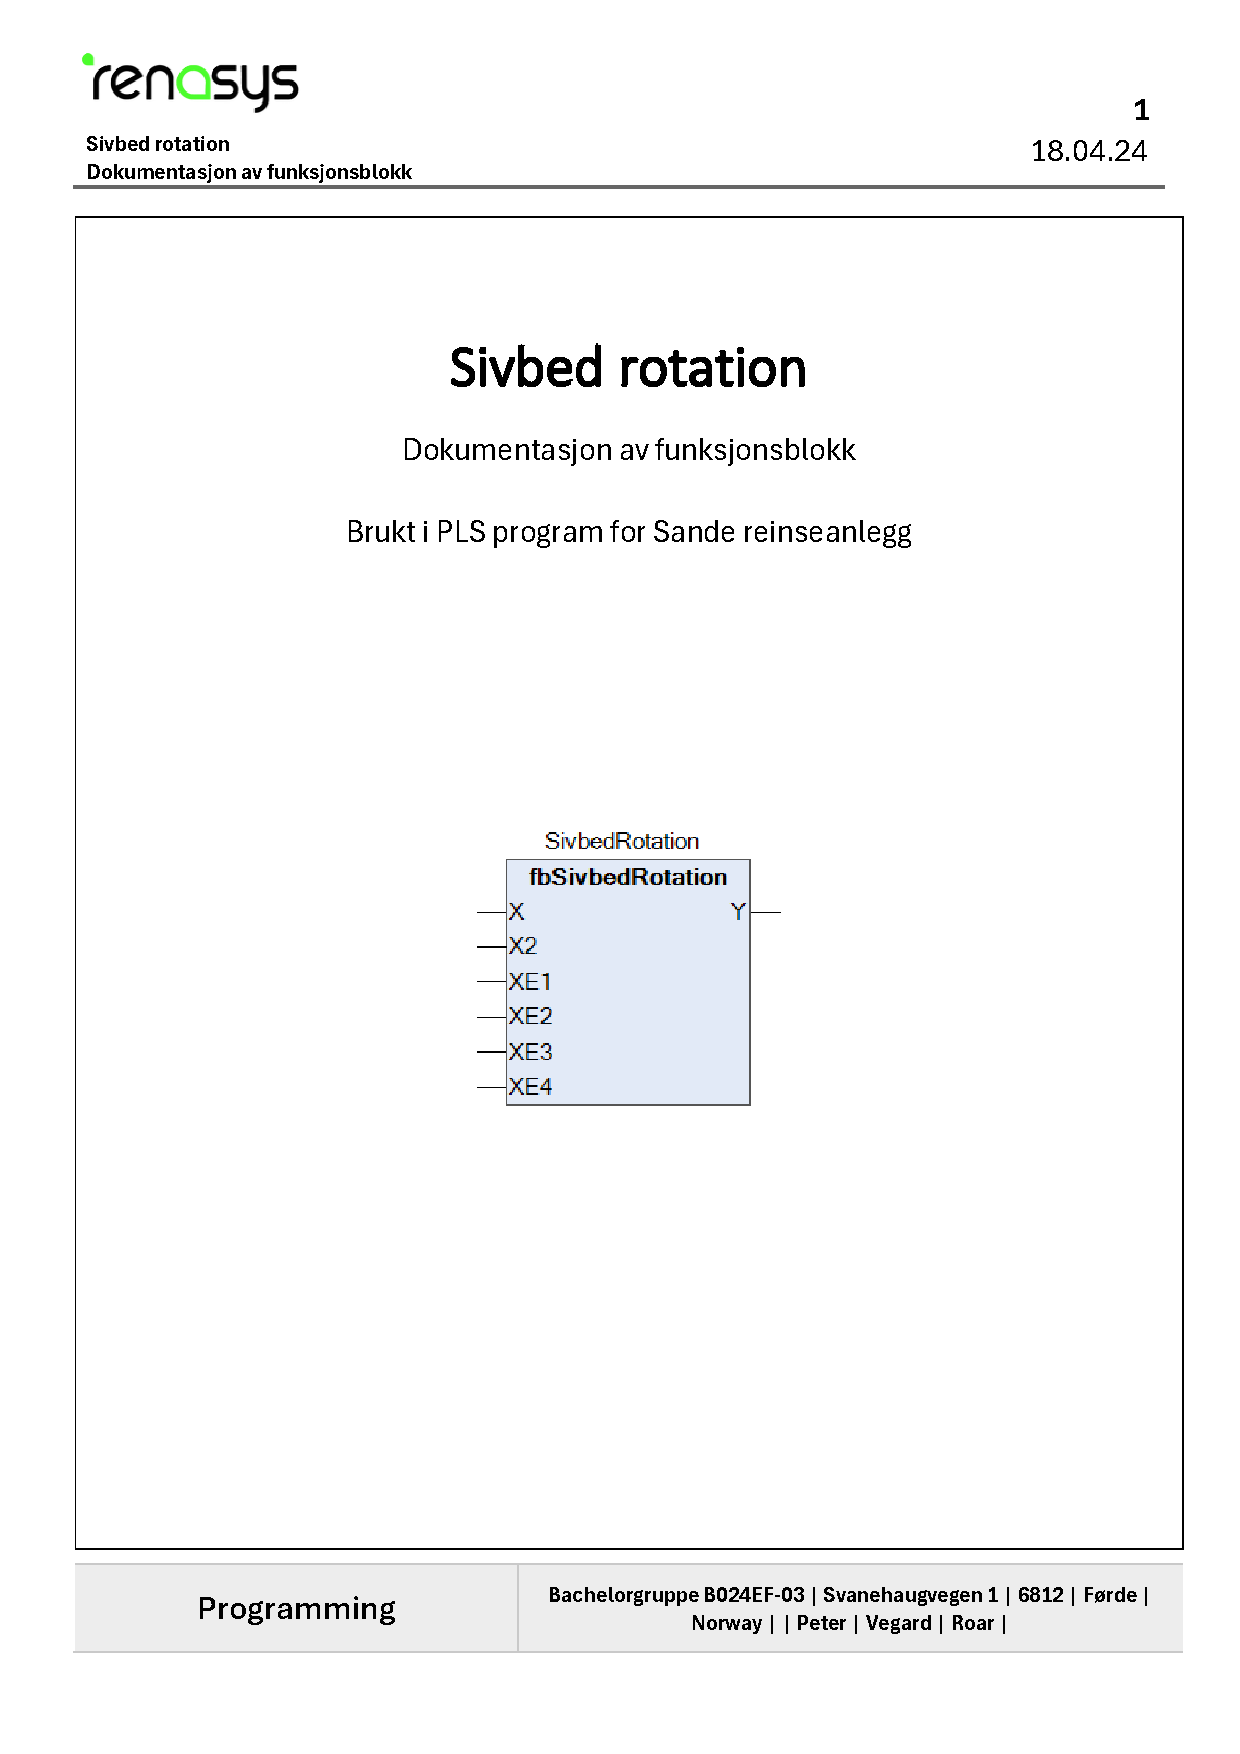
\includepdf[pages=1, scale=0.8, pagecommand={\section{FB Sivbed Rotation}\thispagestyle{fancy}}, fitpaper=true ]{Vedlegg/Funksjons Blokker/fbSivbed Rotation Dokumentasjon.pdf}
\includepdf[pages=2-,scale=0.8, pagecommand={\thispagestyle{fancy}},fitpaper=true]{Vedlegg/Funksjons Blokker/fbSivbed Rotation Dokumentasjon.pdf}
% Swap
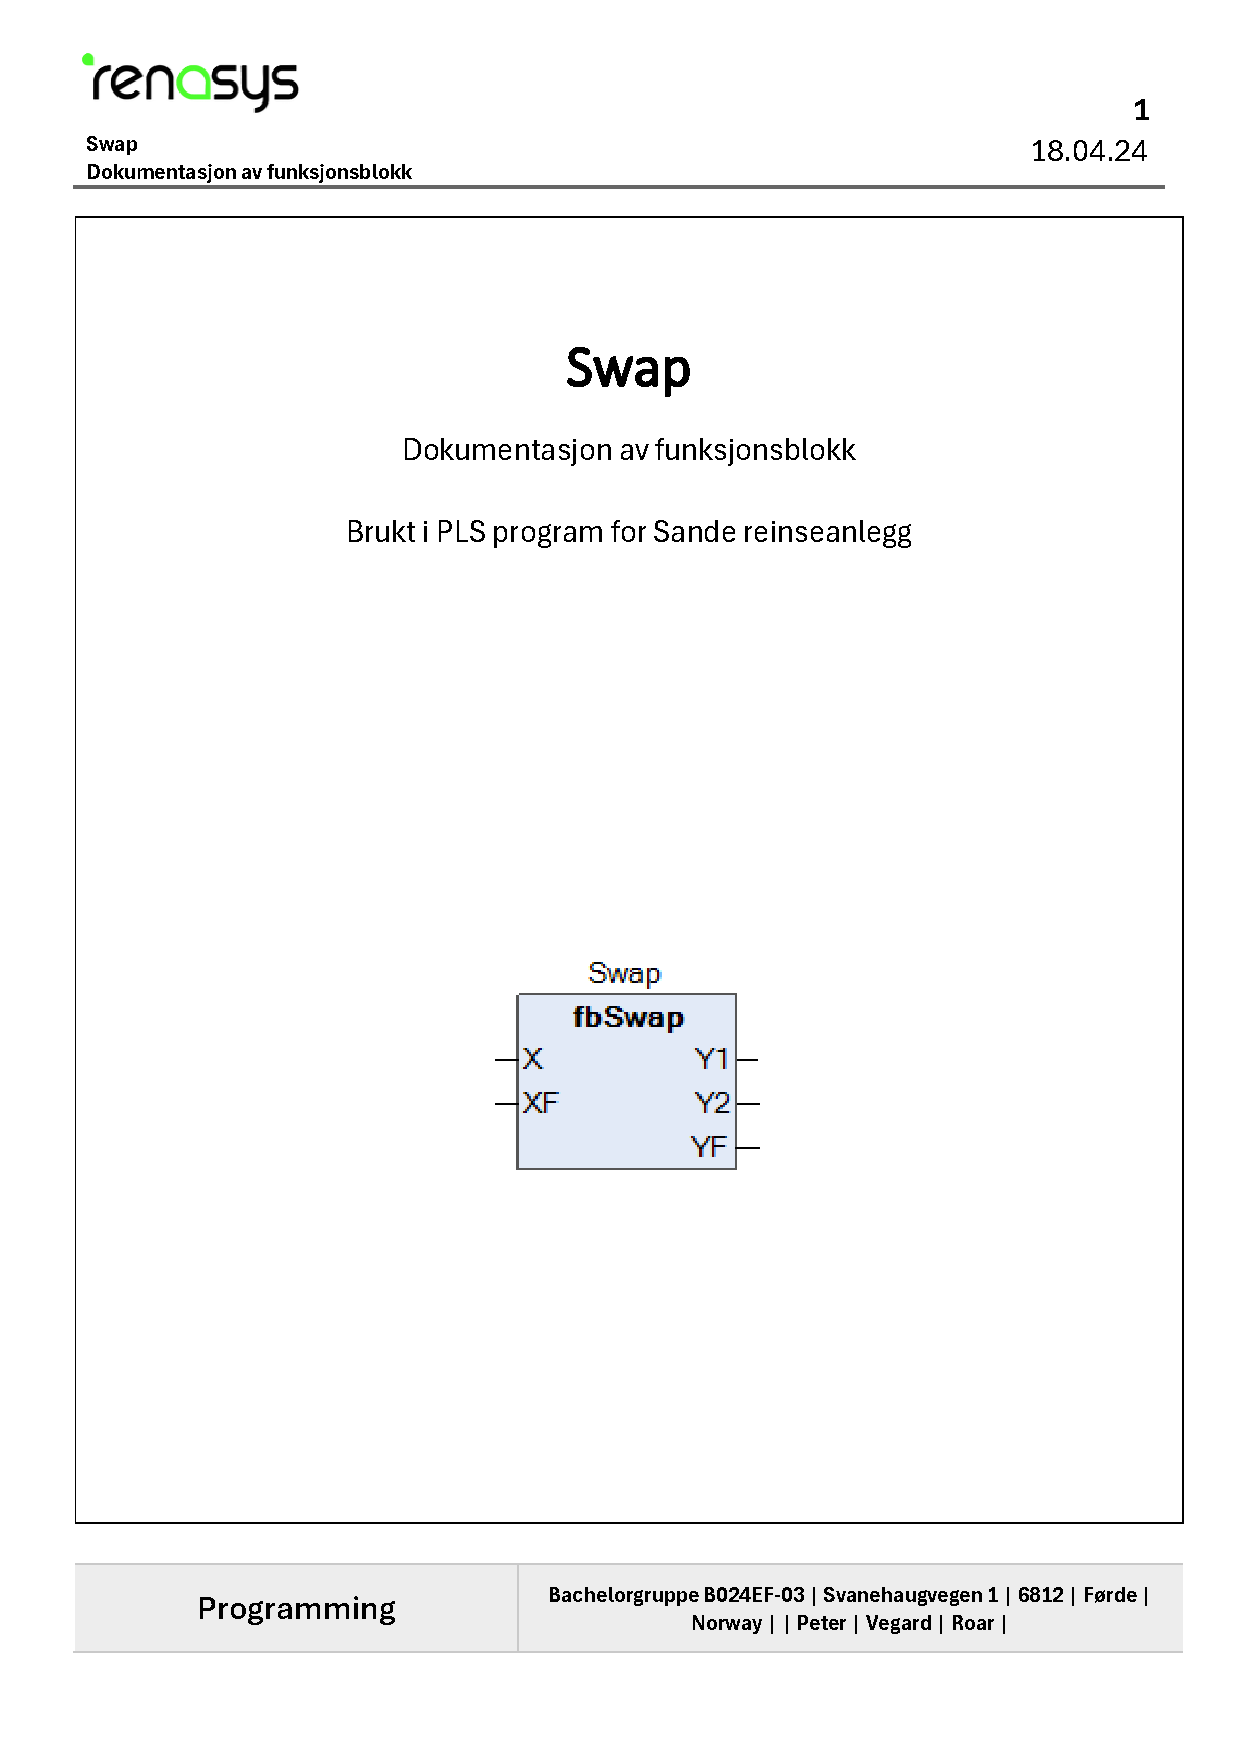
\includepdf[pages=1, scale=0.8, pagecommand={\section{FB Swap}\thispagestyle{fancy}}, fitpaper=true ]{Vedlegg/Funksjons Blokker/fbSwap Dokumentasjon.pdf}
\includepdf[pages=2-,scale=0.8, pagecommand={\thispagestyle{fancy}},fitpaper=true]{Vedlegg/Funksjons Blokker/fbSwap Dokumentasjon.pdf}
% Time Meter
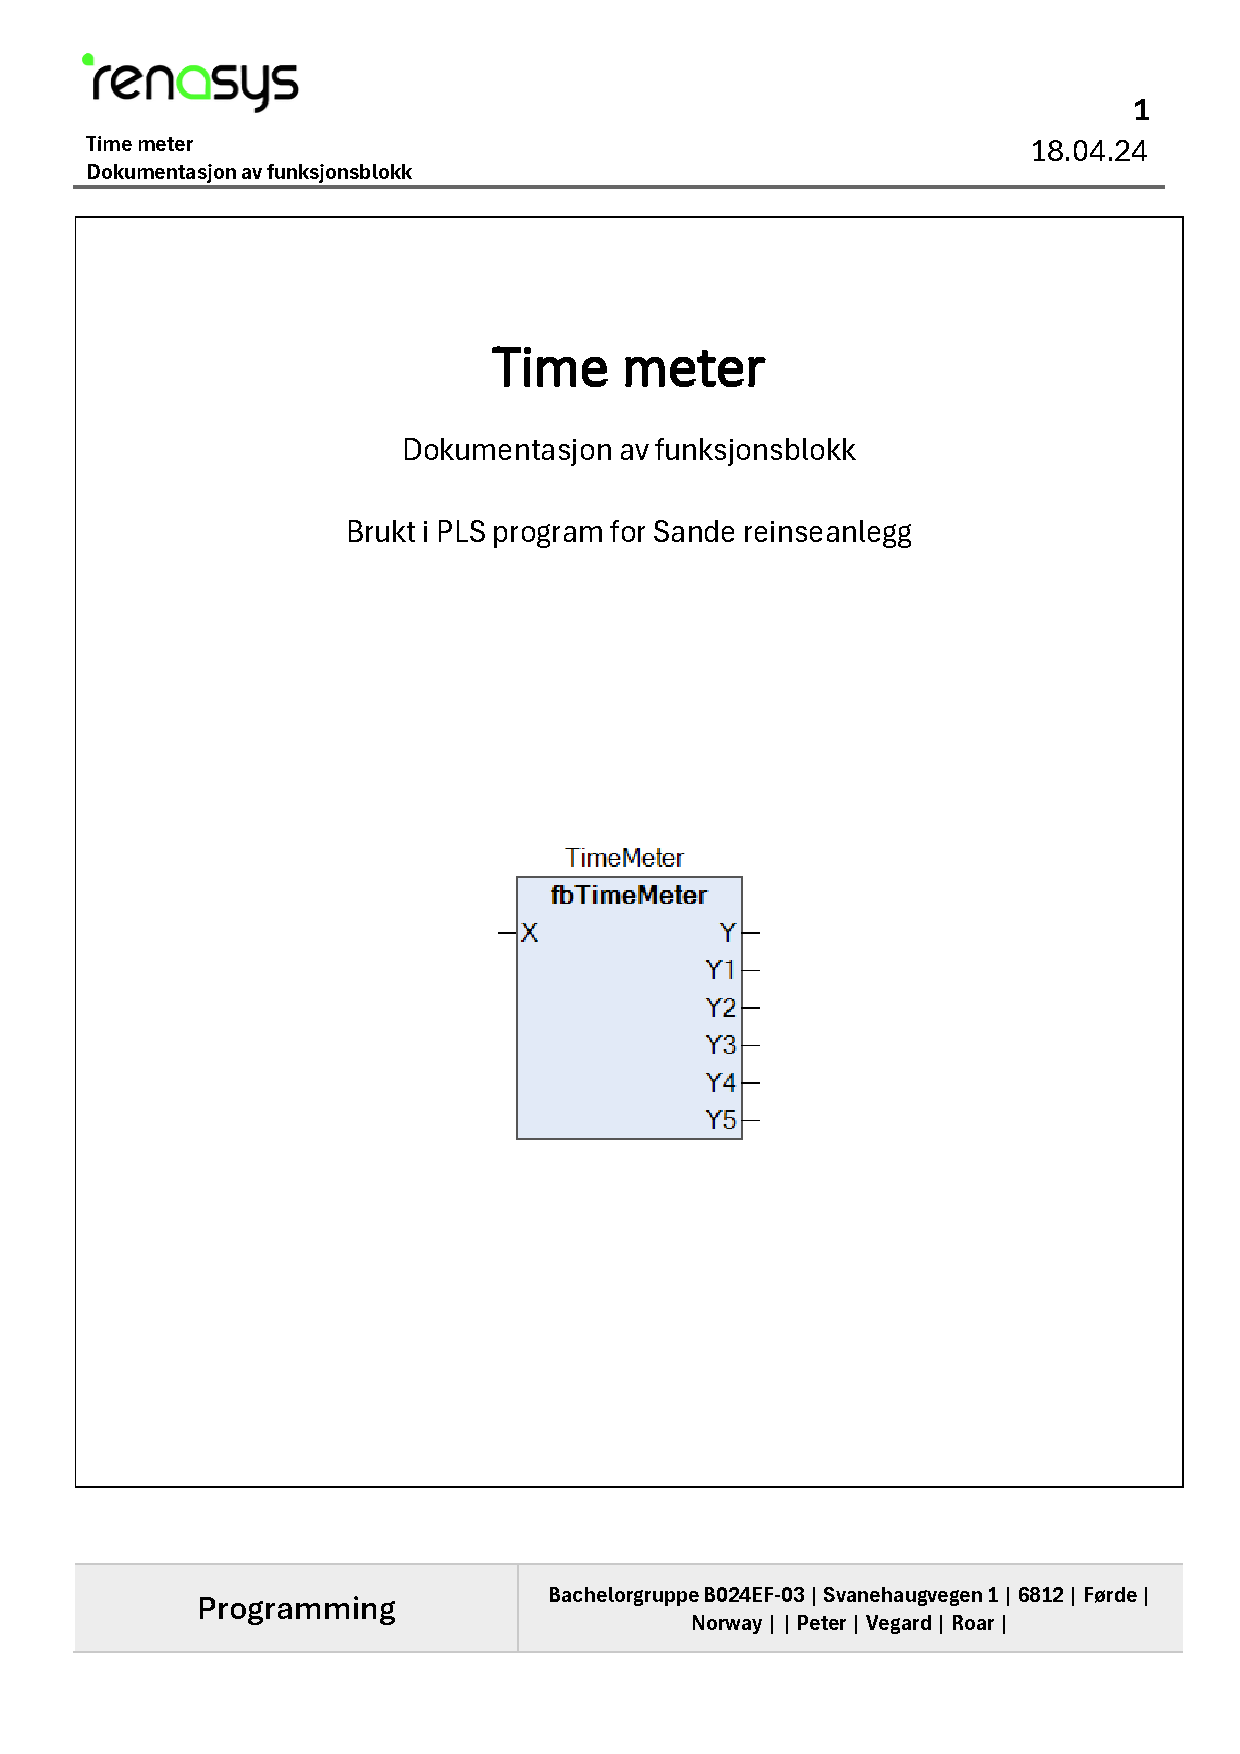
\includepdf[pages=1, scale=0.8, pagecommand={\section{FB Time Meter}\thispagestyle{fancy}}, fitpaper=true ]{Vedlegg/Funksjons Blokker/fbTimeMeter Dokumentasjon.pdf}
\includepdf[pages=2-,scale=0.8, pagecommand={\thispagestyle{fancy}},fitpaper=true]{Vedlegg/Funksjons Blokker/fbTimeMeter Dokumentasjon.pdf}
% Timer
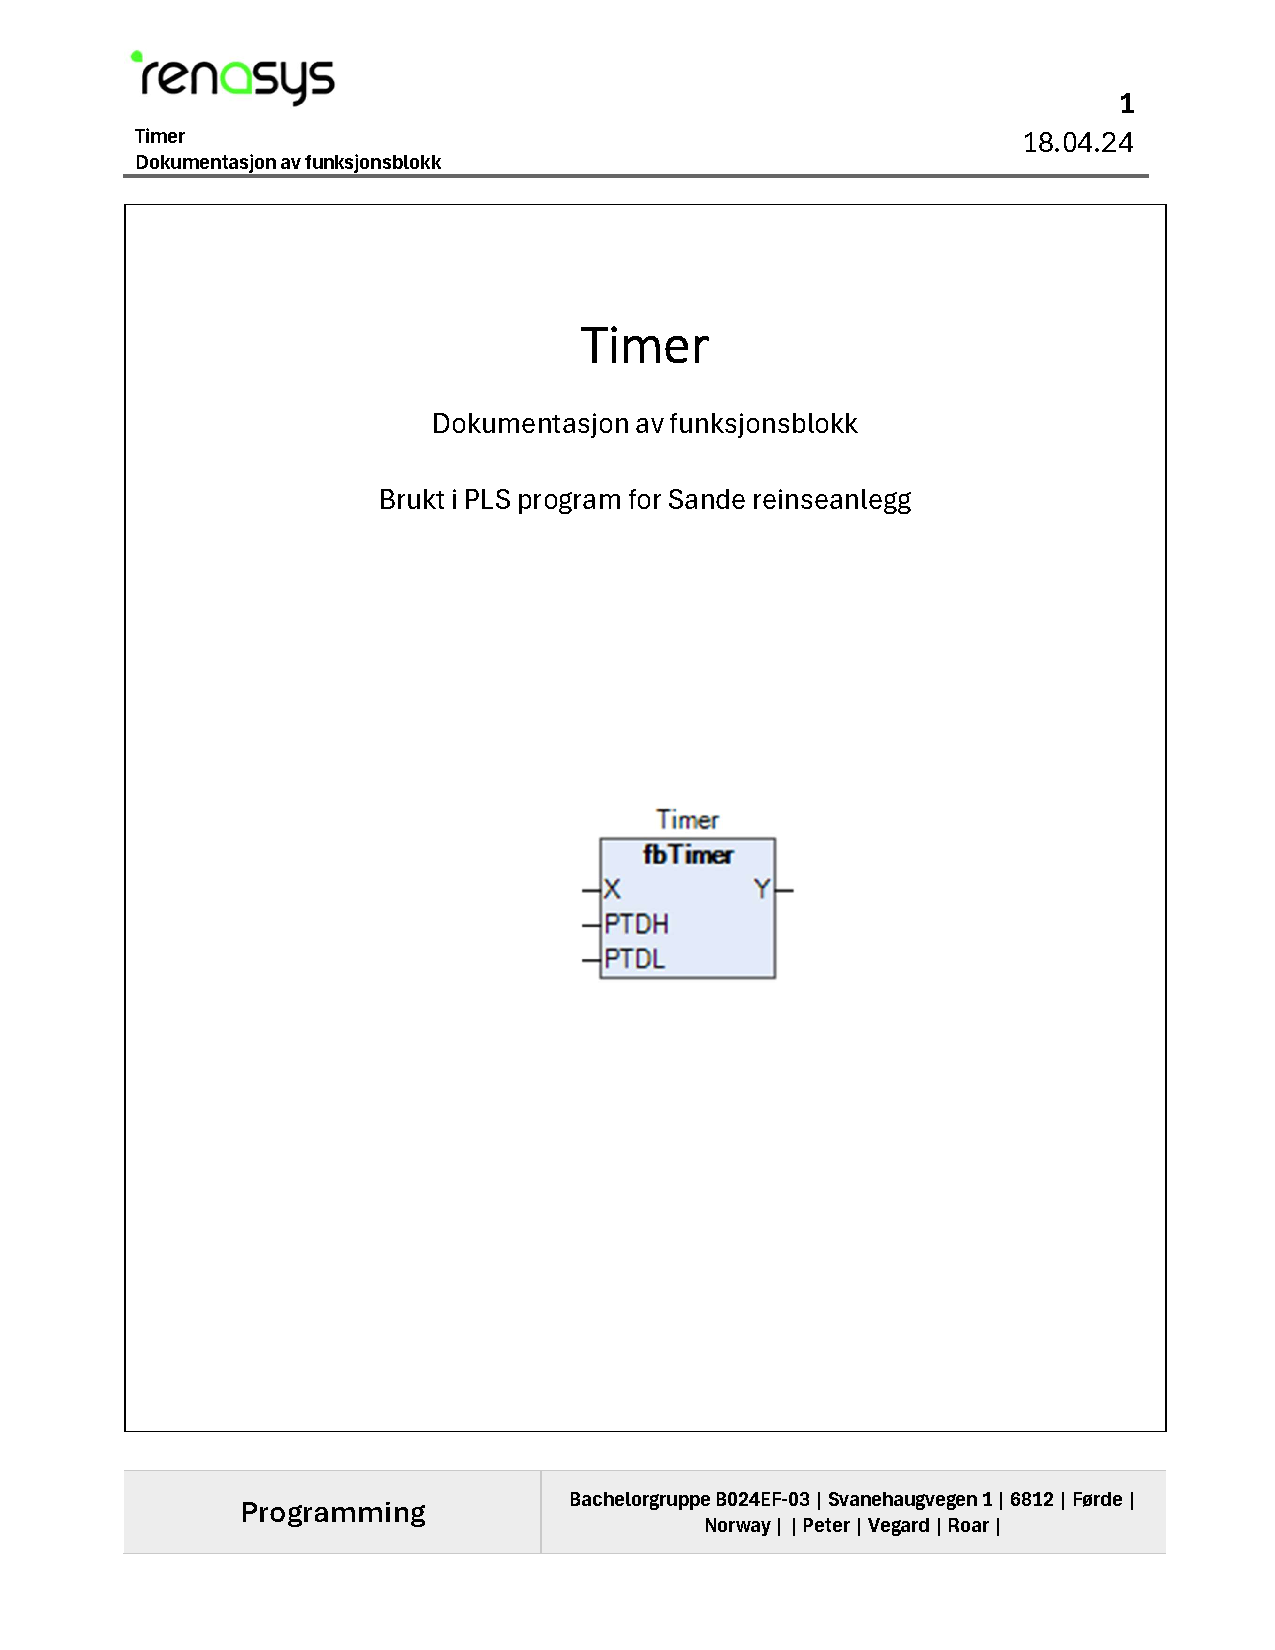
\includepdf[pages=1, scale=0.8, pagecommand={\section{FB Timer}\thispagestyle{fancy}}, fitpaper=true ]{Vedlegg/Funksjons Blokker/fbTimer.pdf}
\includepdf[pages=2-,scale=0.8, pagecommand={\thispagestyle{fancy}},fitpaper=true]{Vedlegg/Funksjons Blokker/fbTimer.pdf}


\chapter{IEC Blokker}
% MB Blokk
% Include only the first page
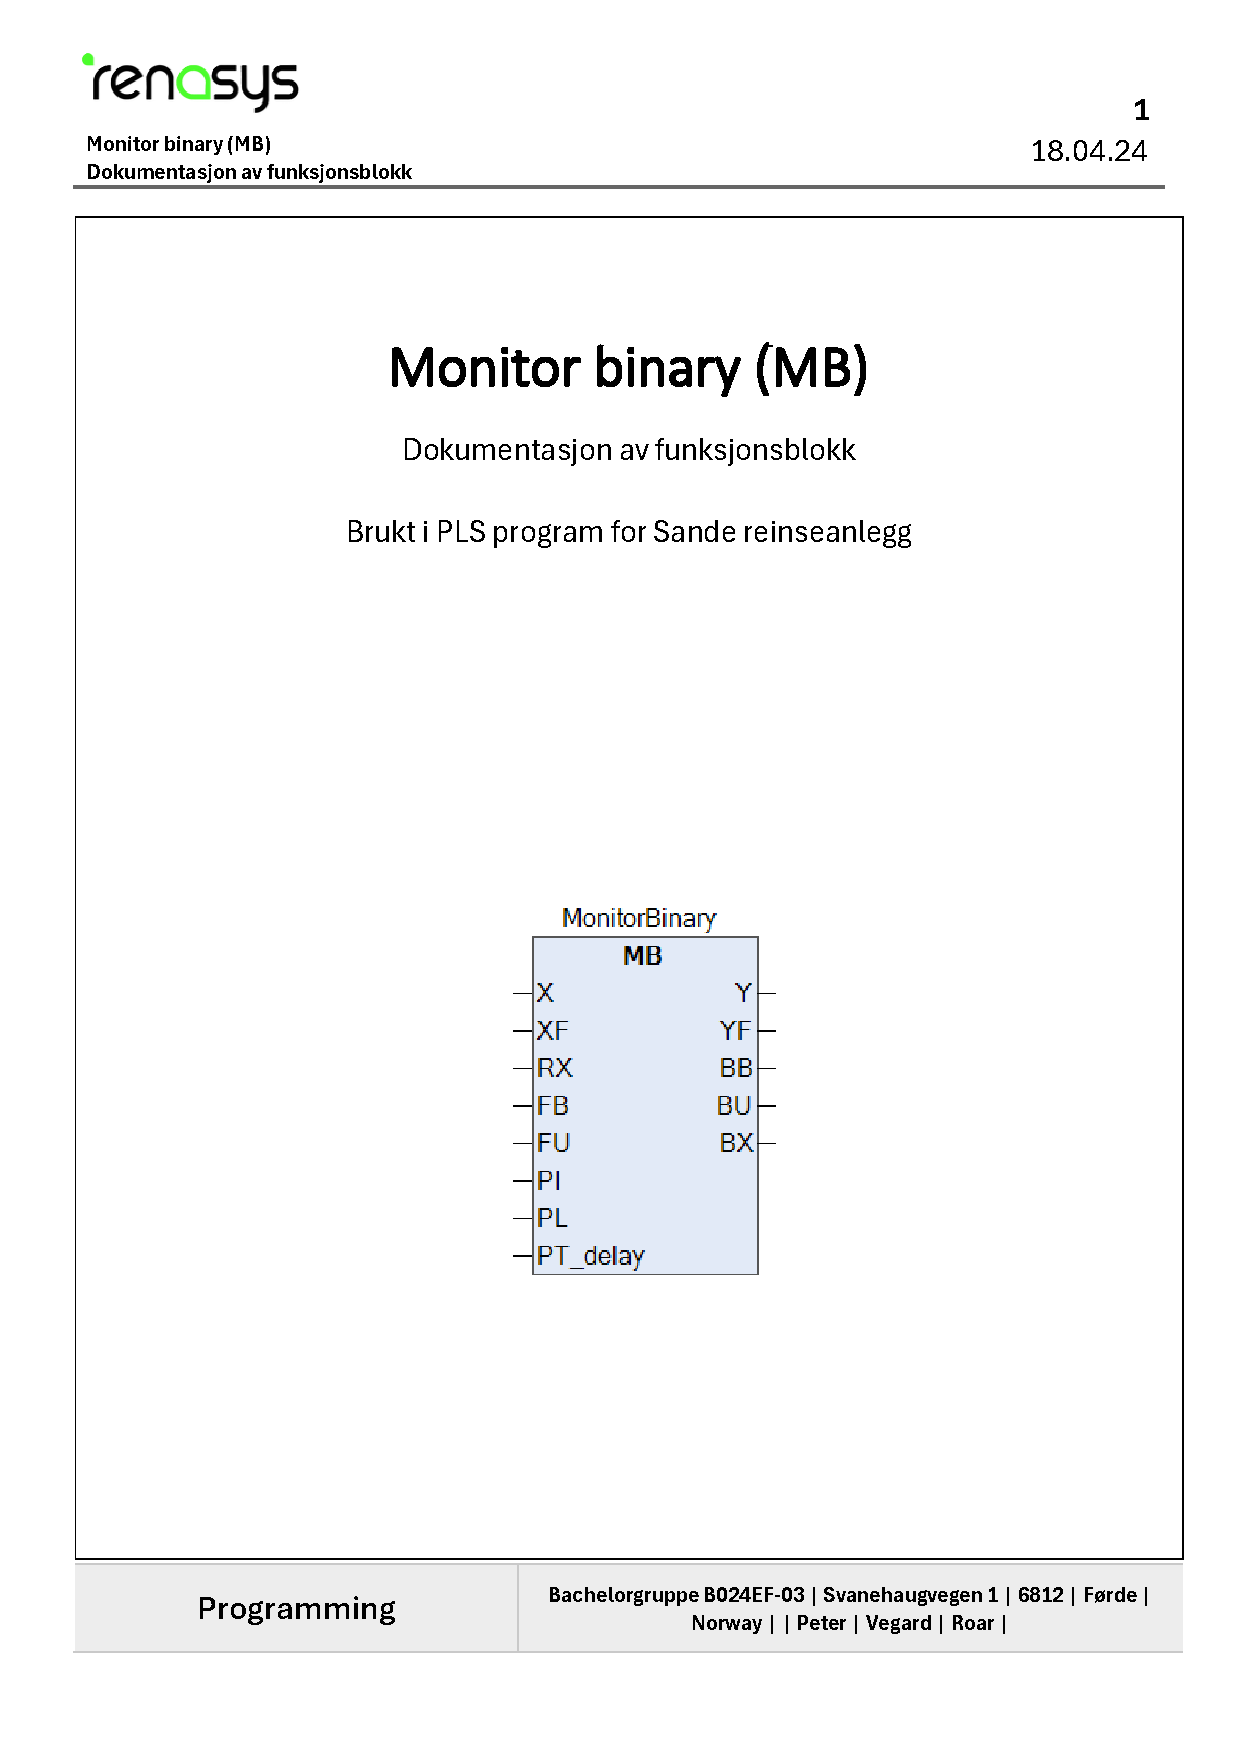
\includepdf[pages=1,scale=0.8, pagecommand={\section{Montor binary}\thispagestyle{fancy}},fitpaper=true]{Vedlegg/IEC Blokker/MB Dokumentasjon.pdf}
% Include the rest of the pages, Starts from the second page to the last, Keep the same scale for all pages
\includepdf[pages=2-, scale=0.8, pagecommand={\thispagestyle{fancy}}, fitpaper=true]{Vedlegg/IEC Blokker/MB Dokumentasjon.pdf}

% MA Blokk
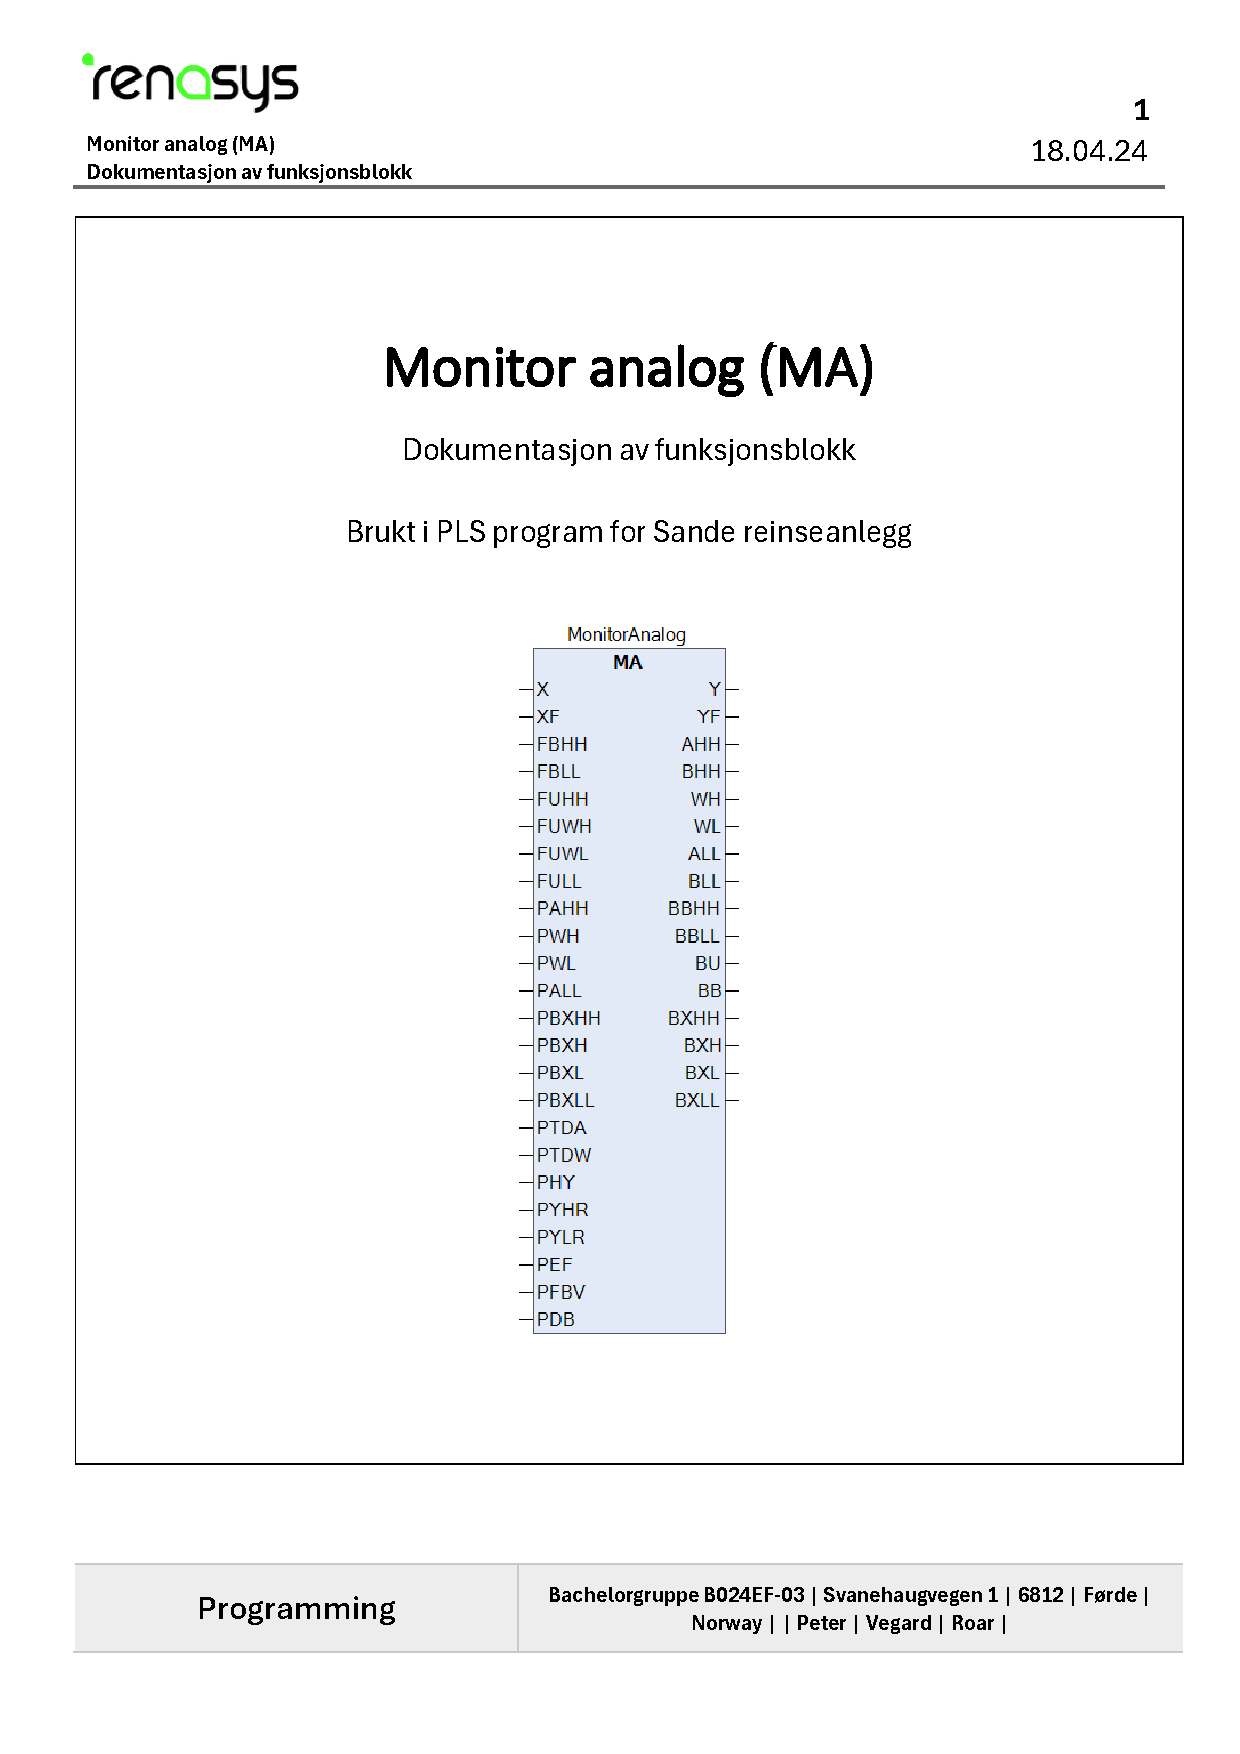
\includepdf[pages=1, scale=0.8, pagecommand={\section{Monitor Analogue}\thispagestyle{fancy}}, fitpaper=true ]{Vedlegg/IEC Blokker/MA Dokumentasjon.pdf}
\includepdf[pages=2-,scale=0.8, pagecommand={\thispagestyle{fancy}},fitpaper=true]{Vedlegg/IEC Blokker/MA Dokumentasjon.pdf}

% SBE Blokk
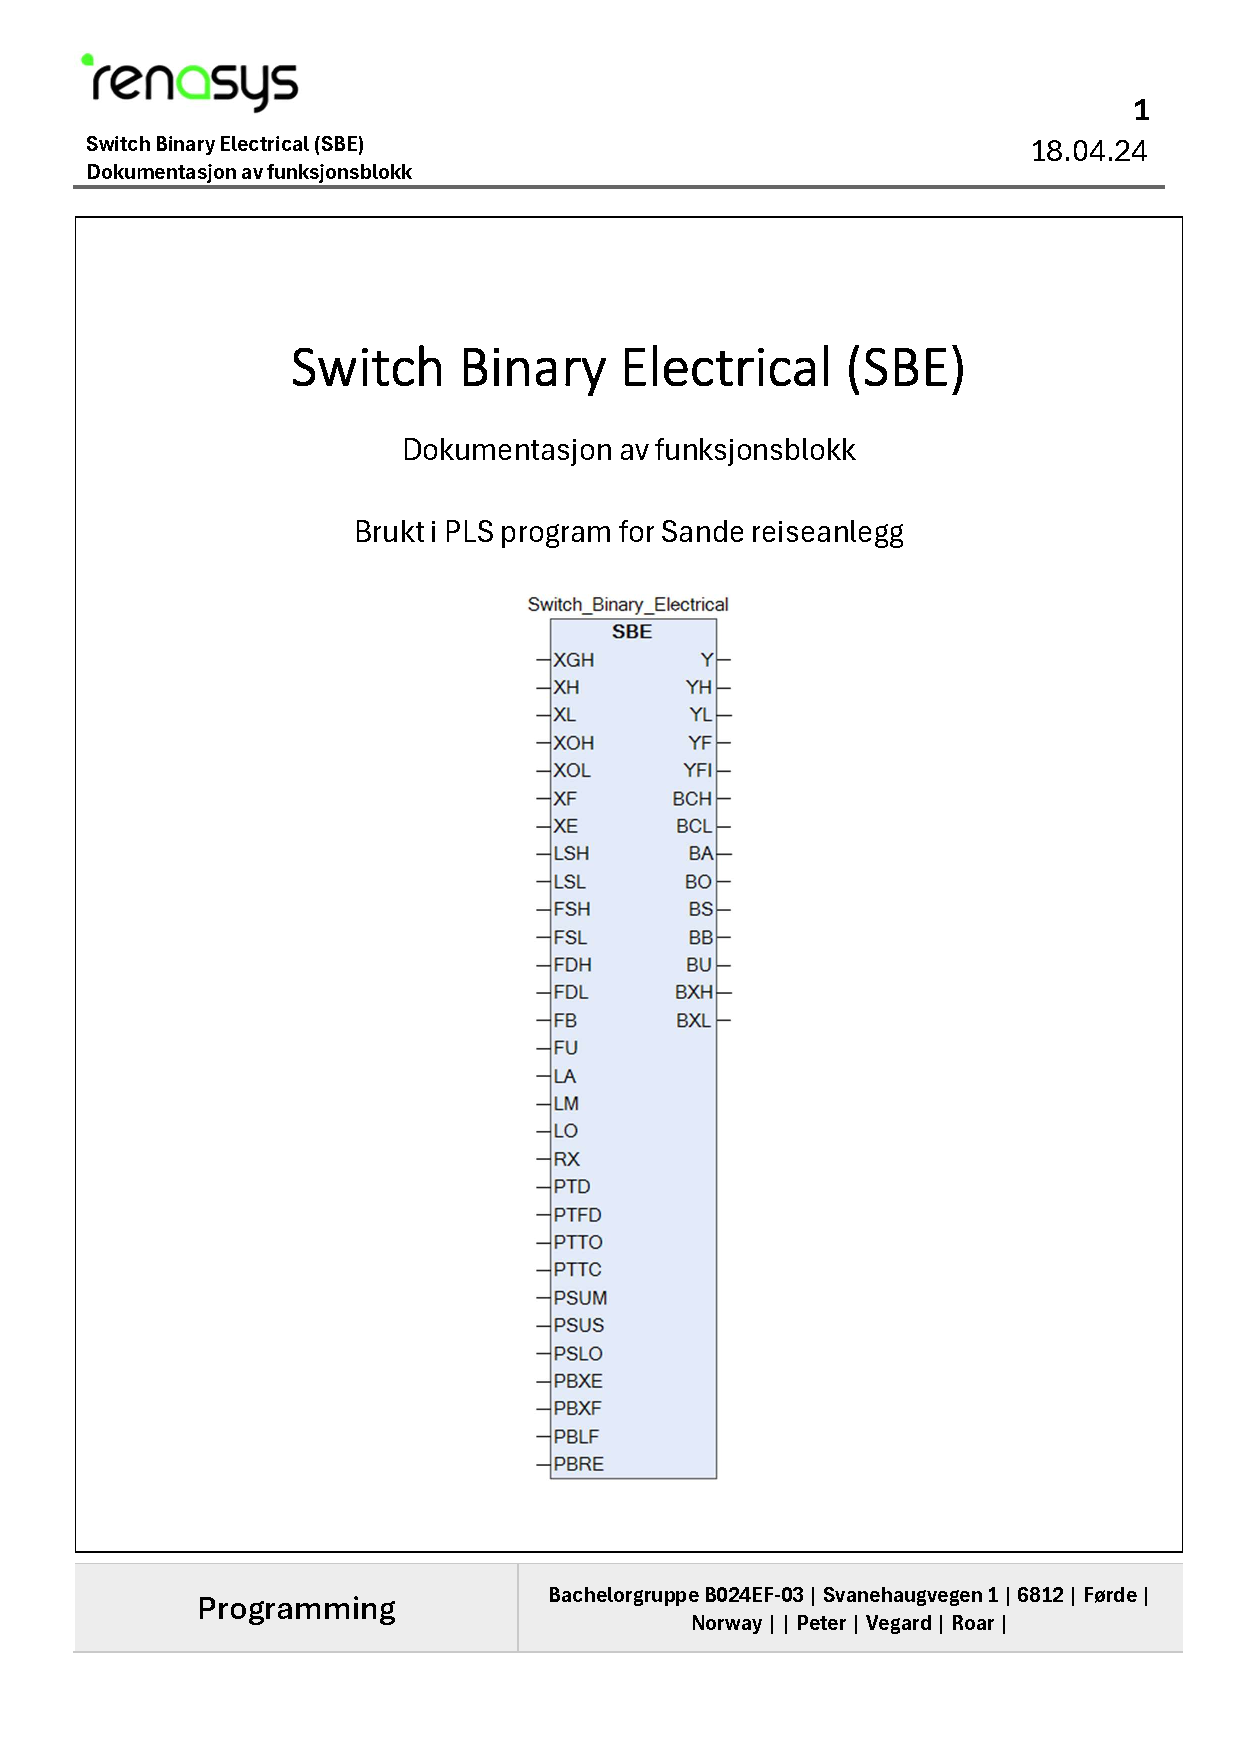
\includepdf[pages=1, scale=0.8, pagecommand={\section{Switch Binary Eletrical}\thispagestyle{fancy}}, fitpaper=true ]{Vedlegg/IEC Blokker/SBE Dokumentasjon.pdf}
\includepdf[pages=2-,scale=0.8, pagecommand={\thispagestyle{fancy}},fitpaper=true]{Vedlegg/IEC Blokker/SBE Dokumentasjon.pdf}

% SBV Blokk
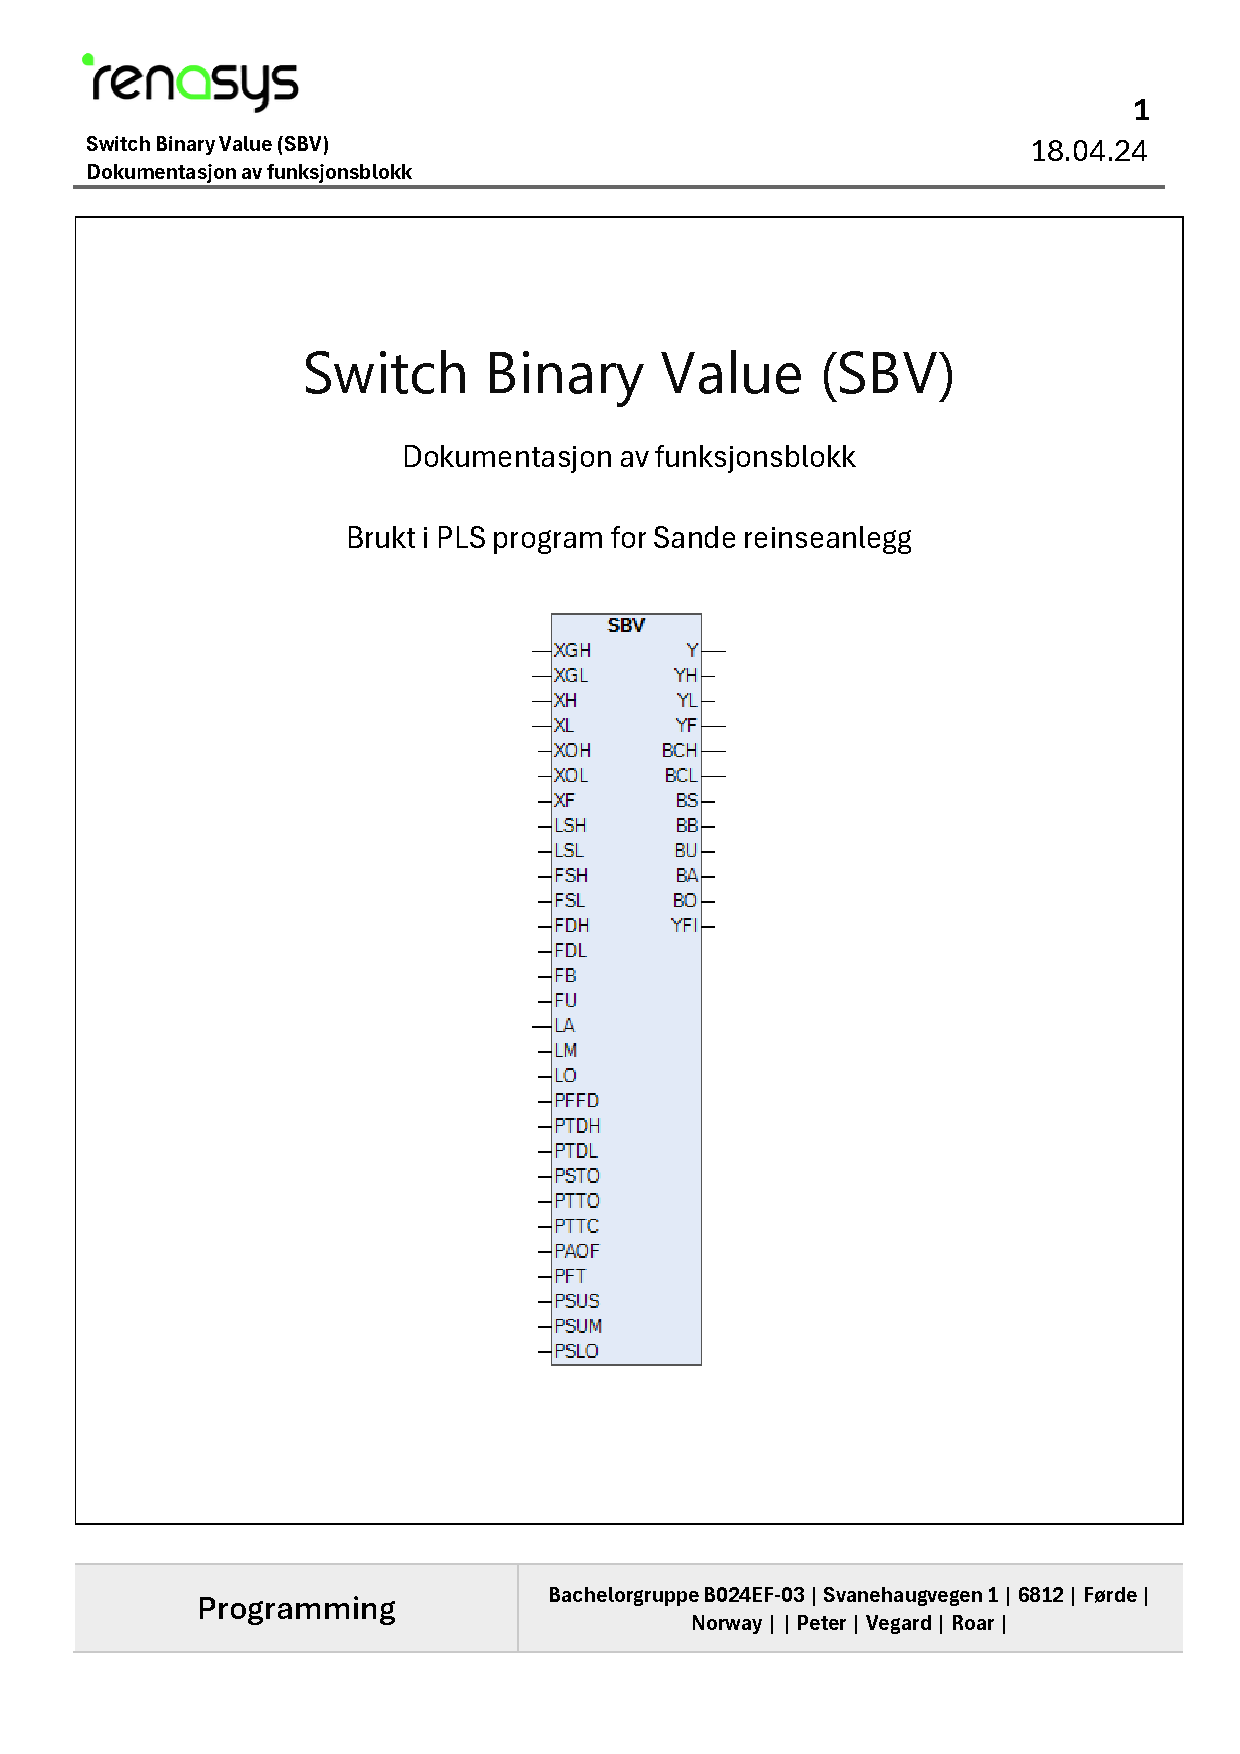
\includepdf[pages=1, scale=0.8, pagecommand={\section{Switch Binary Valve}\thispagestyle{fancy}}, fitpaper=true ]{Vedlegg/IEC Blokker/SBV Dokumentasjon.pdf}
\includepdf[pages=2-,scale=0.8, pagecommand={\thispagestyle{fancy}},fitpaper=true]{Vedlegg/IEC Blokker/SBV Dokumentasjon.pdf}


% ----------- Nytt Kapittel
\chapter{Funksjoner}
% Volume Rektangel
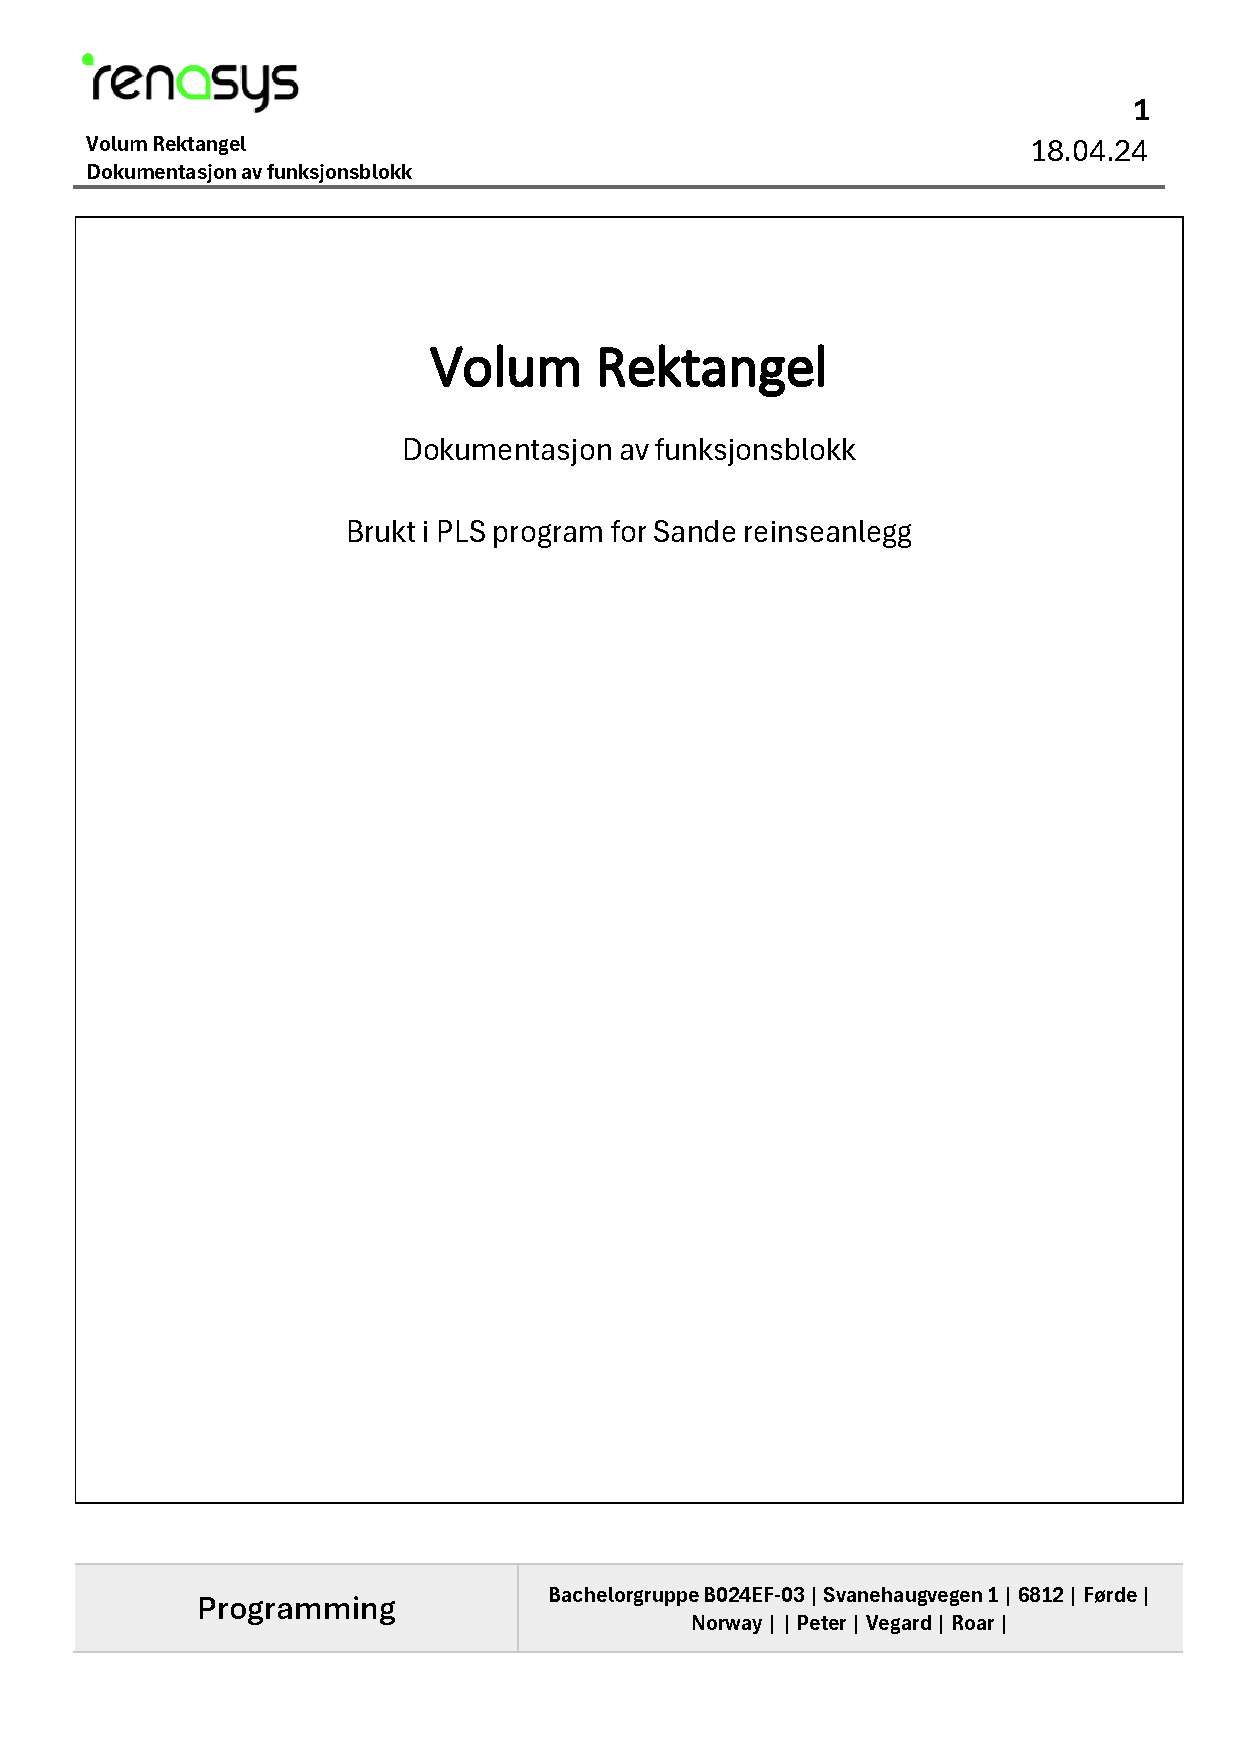
\includepdf[pages=1, scale=0.8, pagecommand={\section{FC Volum rektangel}\thispagestyle{fancy}}, fitpaper=true ]{Vedlegg/Funksjoner/Volume_Rectangle.pdf}
\includepdf[pages=2-,scale=0.8, pagecommand={\thispagestyle{fancy}},fitpaper=true]{Vedlegg/Funksjoner/Volume_Rectangle.pdf}
% Volume Sylinder
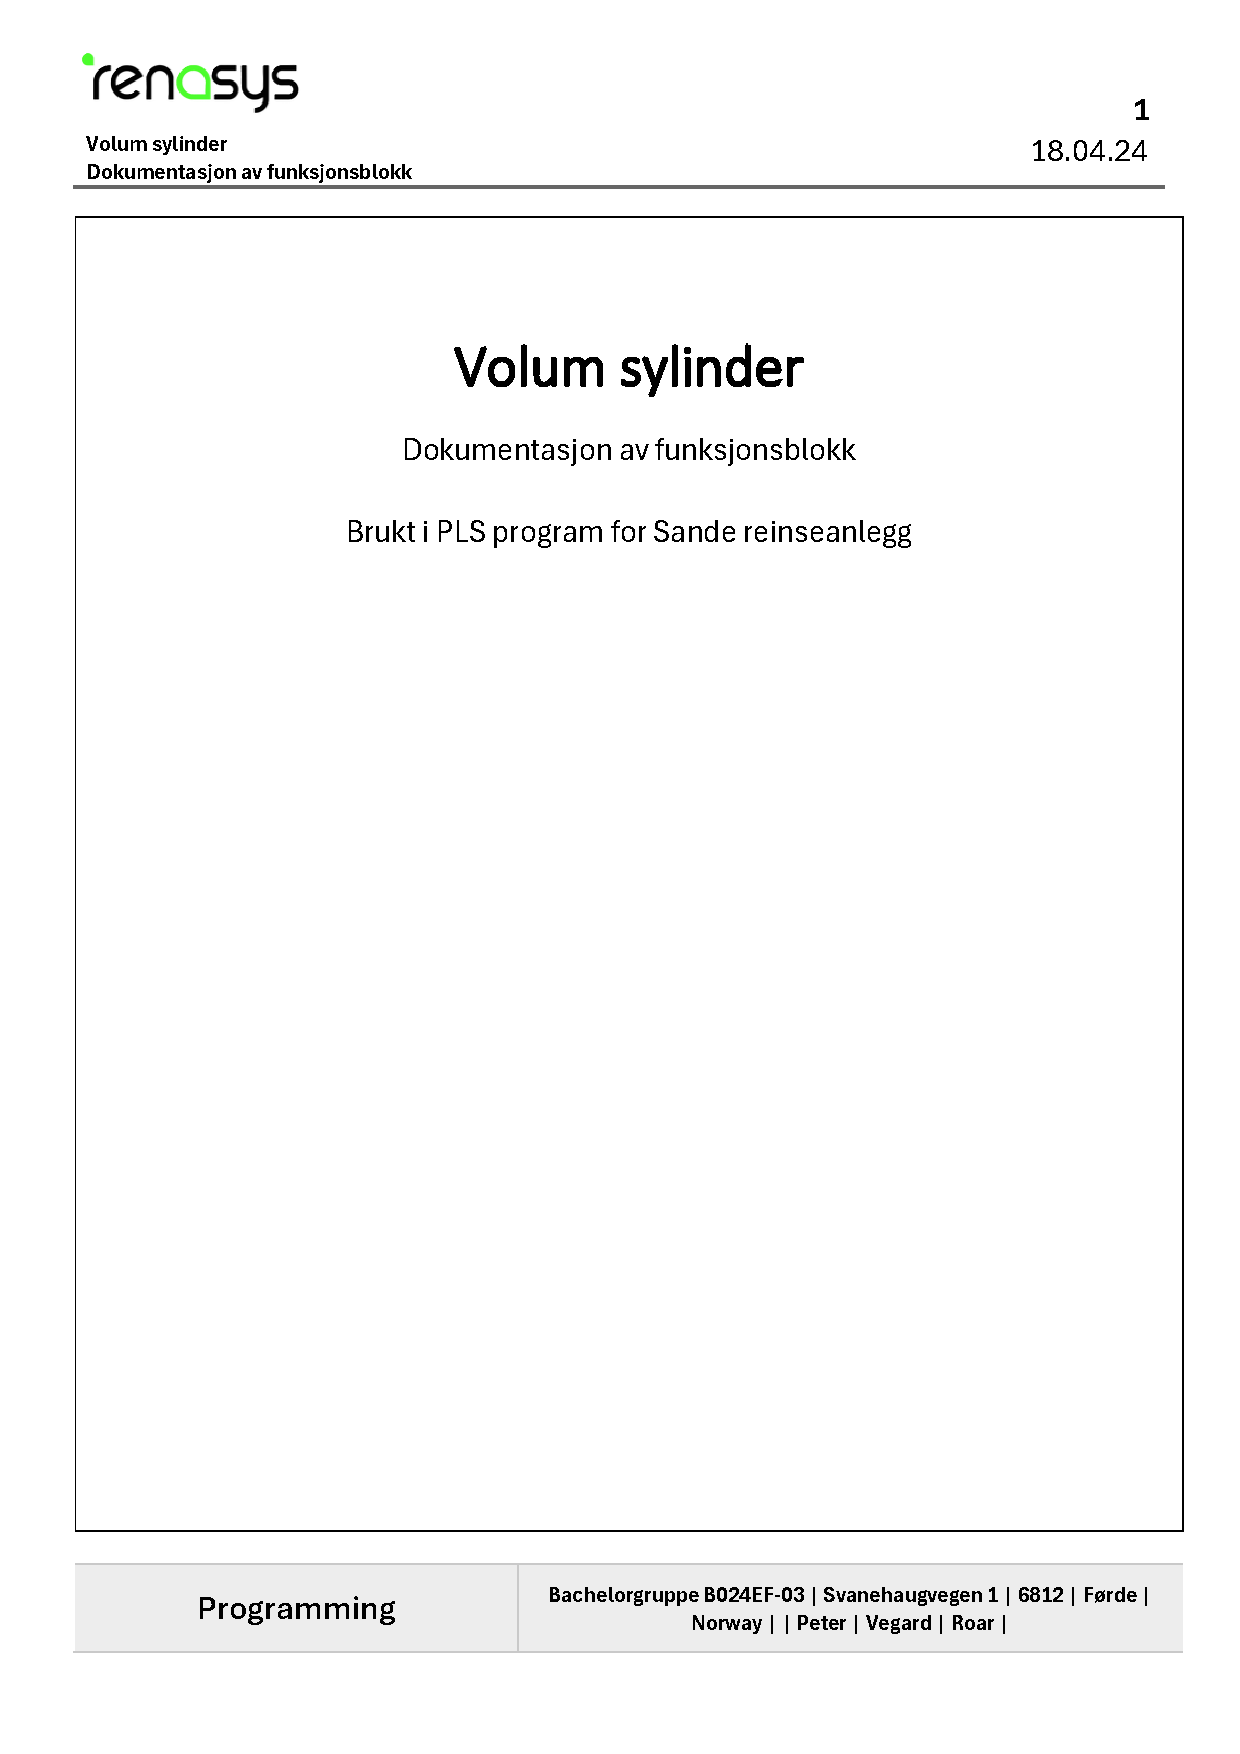
\includepdf[pages=1, scale=0.8, pagecommand={\section{FC Volum Sylinder}\thispagestyle{fancy}}, fitpaper=true ]{Vedlegg/Funksjoner/Volume_Cylinder.pdf}
\includepdf[pages=2-,scale=0.8, pagecommand={\thispagestyle{fancy}},fitpaper=true]{Vedlegg/Funksjoner/Volume_Cylinder.pdf}

% ----------- Nytt Kapittel
\chapter{Alarmlister}

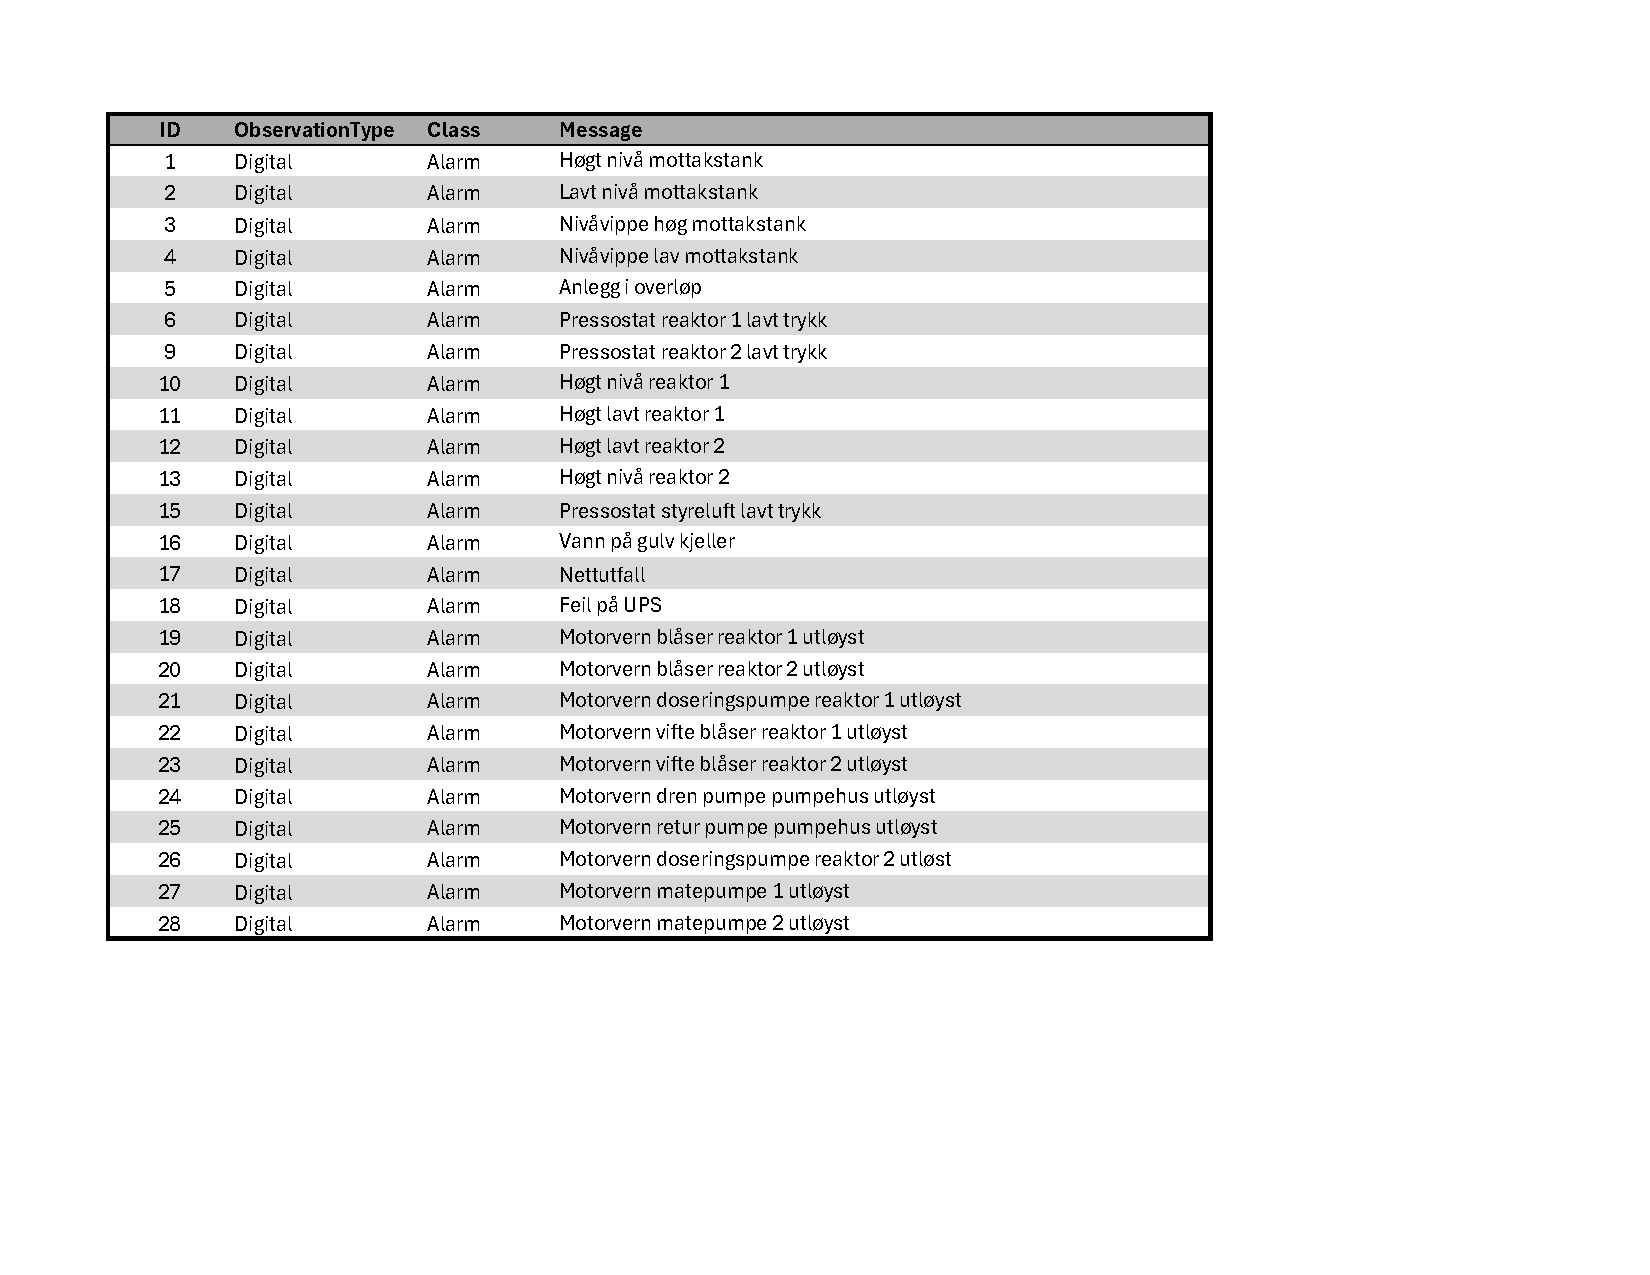
\includepdf[pages=1, scale=0.8, pagecommand={\section{Alarm liste}\thispagestyle{fancy}}, fitpaper=true ]{Vedlegg/AlarmLister/AlarmListe.pdf}

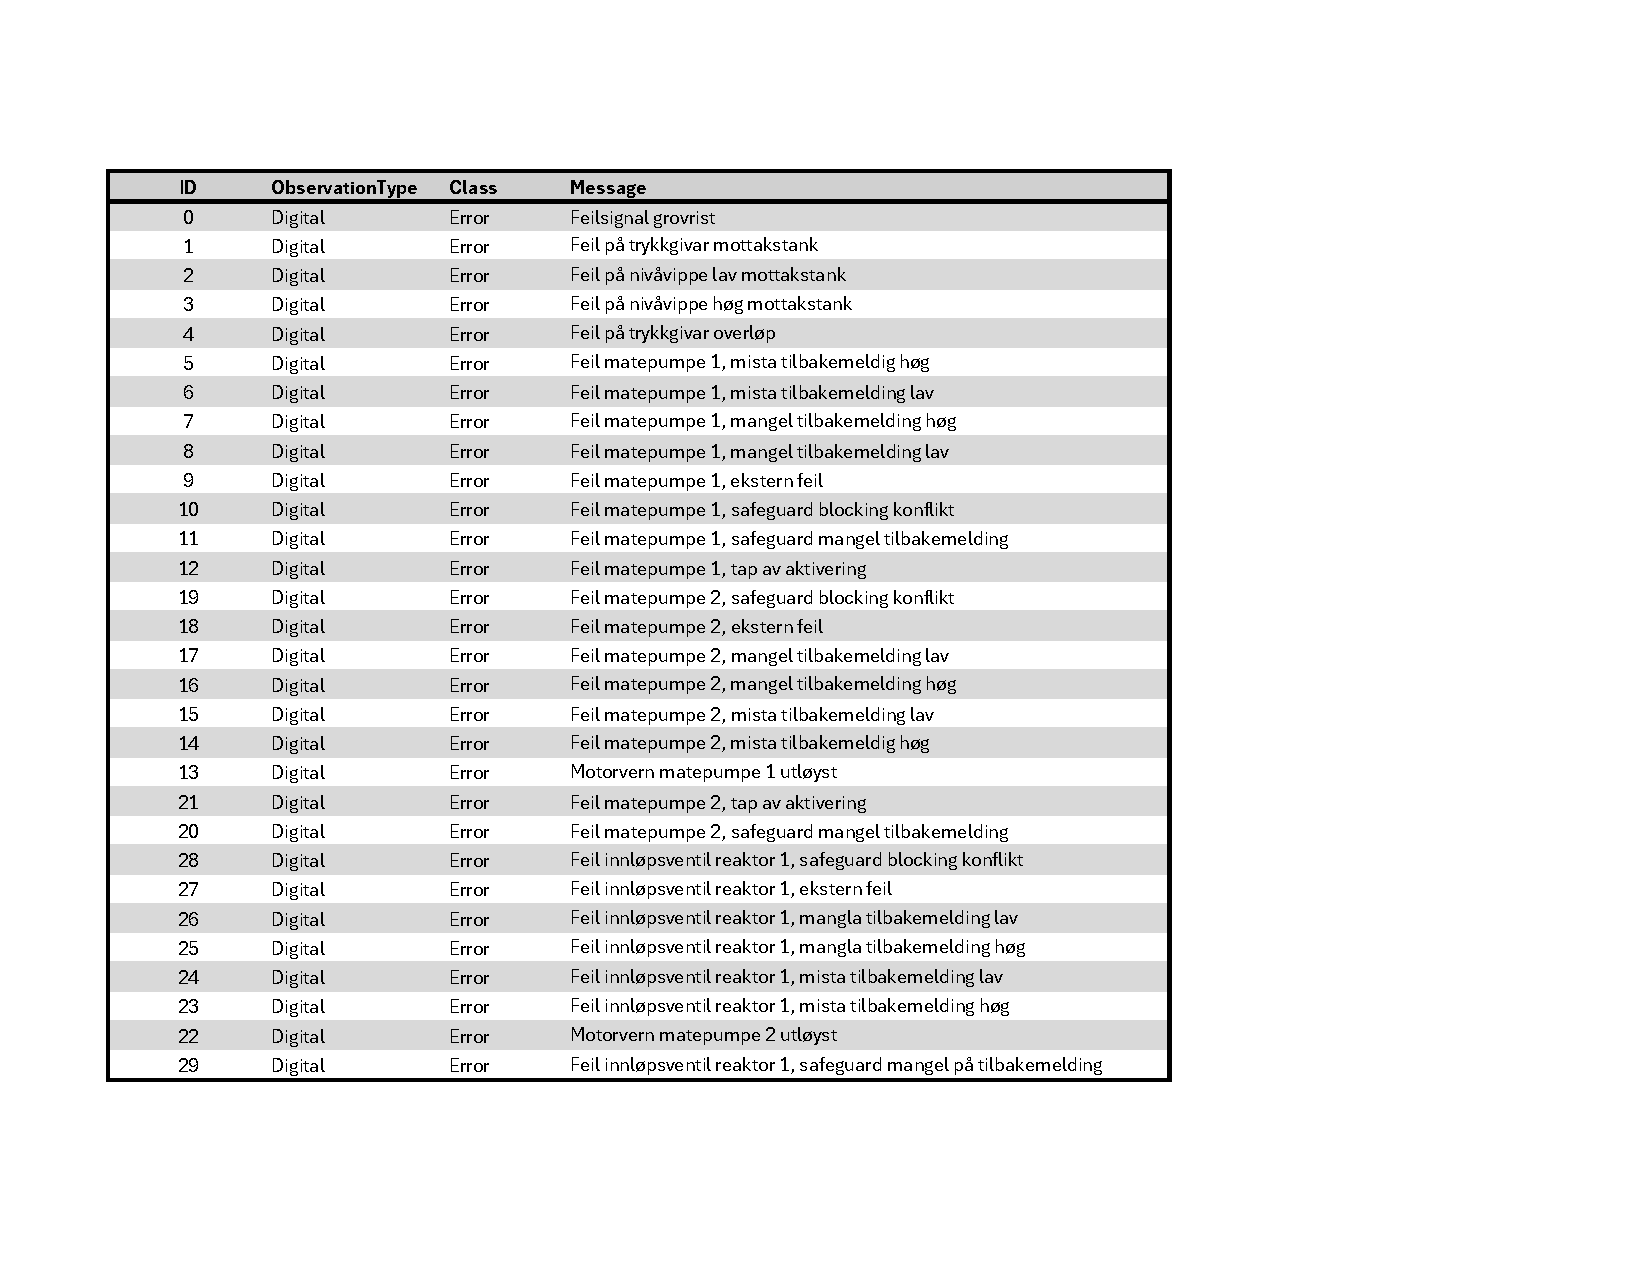
\includepdf[pages=1, scale=0.8, pagecommand={\section{Error liste}\thispagestyle{fancy}}, fitpaper=true ]{Vedlegg/AlarmLister/ErrorListe.pdf}
\includepdf[pages=2-,scale=0.8, pagecommand={\thispagestyle{fancy}},fitpaper=true]{Vedlegg/AlarmLister/ErrorListe.pdf}

% ----------- Nytt Kapittel
% Driftsinstruks Sande

\includepdf[pages=1, scale=0.8, pagecommand={\chapter{Driftsinstruks Orginal}\thispagestyle{fancy}}, fitpaper=true ]{Vedlegg/Driftsinstruks_Sande_RA_Orginal.pdf}
\includepdf[pages=2-,scale=0.8, pagecommand={\thispagestyle{fancy}},fitpaper=true]{Vedlegg/Driftsinstruks_Sande_RA_Orginal.pdf}

% ----------- Nytt Kapittel
% Funksjonsbeskrivelse Sande
\includepdf[pages=1, scale=0.8, pagecommand={\chapter{Funksjonsbeskrivelse}\thispagestyle{fancy}}, fitpaper=true ]{Vedlegg/Funksjonsbeskrivelse.pdf}
\includepdf[pages=2-,scale=0.8, pagecommand={\thispagestyle{fancy}},fitpaper=true]{Vedlegg/Funksjonsbeskrivelse.pdf}

% ----------- Nytt Kapittel
% SCD Diagrammer

{\raggedright
\chapter{Sekvensar}\par
}
%\includepdf[pages=1, angle=90, pagecommand={\section{Tilstand Pause}\thispagestyle{fancy}}, fitpaper=true]{Vedlegg/SCD.pdf}
%\includepdf[pages=2, angle=90, pagecommand={\section{Tilstand Innpumping}\thispagestyle{fancy}}, fitpaper=true]{Vedlegg/SCD.pdf}
%\includepdf[pages=3, angle=90, pagecommand={\section{Tilstand Reaksjon}\thispagestyle{fancy}}, fitpaper=true]{Vedlegg/SCD.pdf}
%\includepdf[pages=4, angle=90, pagecommand={\section{Tilstand Sedimentering}\thispagestyle{fancy}}, fitpaper=true]{Vedlegg/SCD.pdf}
%\includepdf[pages=5, angle=90, pagecommand={\section{Tilstand Uttapping}\thispagestyle{fancy}}, fitpaper=true]{Vedlegg/SCD.pdf}
%\includepdf[pages=6, angle=90, pagecommand={\section{Tilstand Felles Styring}\thispagestyle{fancy}}, fitpaper=true]{Vedlegg/SCD.pdf}

%\section{Tilstand Pause1}
\thispagestyle{plain}
{
\raggedright
\section{Tilstand Pause}\par
}
\thispagestyle{fancy}
%\leftalignedsection{Tilstand Pause}
\begin{adjustwidth}{-3cm}{-3cm}
\begin{tikzpicture}[remember picture, overlay]
    % Include the PDF page rotated, positioned at the center of the page
    % Gammel scale for alle SCD var scale=0.36 for fullpage scale
    \node[inner sep=0pt] at (current page.center) {
        \includegraphics[page=1,angle=90, scale=0.92, keepaspectratio]{Vedlegg/SCD_OppdatertAHH-Gate.pdf}
    };
\end{tikzpicture}
\end{adjustwidth}
\newpage
\section{Tilstand Innpumping}
\begin{tikzpicture}[remember picture, overlay]
    % Include the PDF page rotated, positioned at the center of the page
    \node[inner sep=0pt] at (current page.center) {
        \includegraphics[page=2,angle=90, scale=0.92, keepaspectratio]{Vedlegg/SCD_OppdatertAHH-Gate.pdf}
    };
\end{tikzpicture}
\newpage
\section{Tilstand Reaksjon}
\begin{tikzpicture}[remember picture, overlay]
    % Include the PDF page rotated, positioned at the center of the page
    \node[inner sep=0pt] at (current page.center) {
        \includegraphics[page=3,angle=90, scale=0.92, keepaspectratio]{Vedlegg/SCD_OppdatertAHH-Gate.pdf}
    };
\end{tikzpicture}
\newpage
\section{Tilstand Sedimentering}
\begin{tikzpicture}[remember picture, overlay]
    % Include the PDF page rotated, positioned at the center of the page
    \node[inner sep=0pt] at (current page.center) {
        \includegraphics[page=4,angle=90, scale=0.92, keepaspectratio]{Vedlegg/SCD_OppdatertAHH-Gate.pdf}
    };
\end{tikzpicture}
\newpage
\section{Tilstand Uttapping}
\begin{tikzpicture}[remember picture, overlay]
    % Include the PDF page rotated, positioned at the center of the page
    \node[inner sep=0pt] at (current page.center) {
        \includegraphics[page=5,angle=90, scale=0.90, keepaspectratio]{Vedlegg/SCD_OppdatertAHH-Gate.pdf}
    };
\end{tikzpicture}
\newpage
\section{Tilstand Felles Styring}
\begin{tikzpicture}[remember picture, overlay]
    % Include the PDF page rotated, positioned at the center of the page
    \node[inner sep=0pt] at (current page.center) {
        \includegraphics[page=6,angle=90, scale=0.92, keepaspectratio]{Vedlegg/SCD_OppdatertAHH-Gate.pdf}
    };
\end{tikzpicture}

% ----------- Nytt Kapittel VEDLEGG KOMPONENTDOKUMENTASJON

% Blåser
\includepdf[pages=1, scale=0.75, pagecommand={\chapter{Manualer}\section{Cat blower}\thispagestyle{fancy}}, fitpaper=true ]{Vedlegg/Komponentvedlegg/Blåser/Cat_Blowers_S20_03D08C.pdf}
\includepdf[pages=2-,scale=0.8, pagecommand={\thispagestyle{fancy}},fitpaper=true]{Vedlegg/Komponentvedlegg/Blåser/Cat_Blowers_S20_03D08C.pdf}

\includepdf[pages=1, scale=0.75, pagecommand={\section{cat Robox}\thispagestyle{fancy}}, fitpaper=true ]{Vedlegg/Komponentvedlegg/Blåser/cat-robox-lobe-and-robox-screw-s20-w08-2d20-c-uk.pdf}
\includepdf[pages=2-,scale=0.8, pagecommand={\thispagestyle{fancy}},fitpaper=true]{Vedlegg/Komponentvedlegg/Blåser/cat-robox-lobe-and-robox-screw-s20-w08-2d20-c-uk.pdf}

%Doseringspumpe
\includepdf[pages=1,scale=0.8, pagecommand={\section{Doseringspumpe}\thispagestyle{fancy}},fitpaper=true]{Vedlegg/Komponentvedlegg/Doseringspumpe/bomba membrana coagulante.pdf}
\includepdf[pages=2-,scale=0.8, pagecommand={\thispagestyle{fancy}},fitpaper=true]{Vedlegg/Komponentvedlegg/Doseringspumpe/bomba membrana coagulante.pdf}

%Huber
\includepdf[pages=1,scale=0.8, pagecommand={\section{Huber}\thispagestyle{fancy}},fitpaper=true]{Vedlegg/Komponentvedlegg/Huber/d_keram30-huber.pdf}
\includepdf[pages=2-,scale=0.8, pagecommand={\thispagestyle{fancy}},fitpaper=true]{Vedlegg/Komponentvedlegg/Huber/d_keram30-huber.pdf}

%Motor
\includepdf[pages=1,scale=0.75, pagecommand={\section{Motor}\thispagestyle{fancy}},fitpaper=true]{Vedlegg/Komponentvedlegg/Motor/p-7101-bgm.pdf}
\includepdf[pages=2-,scale=0.8, pagecommand={\thispagestyle{fancy}},fitpaper=true]{Vedlegg/Komponentvedlegg/Motor/p-7101-bgm.pdf}

%Pumpe
\includepdf[pages=1,scale=0.8, pagecommand={\section{Pumpe}\thispagestyle{fancy}},fitpaper=true]{Vedlegg/Komponentvedlegg/Pumpe/flygt-n-pump-brochure-896876.pdf}
\includepdf[pages=2-,scale=0.8, pagecommand={\thispagestyle{fancy}},fitpaper=true]{Vedlegg/Komponentvedlegg/Pumpe/flygt-n-pump-brochure-896876.pdf}

%Transmitter
\includepdf[pages=1,scale=0.8, pagecommand={\section{Transmitter MJK}\thispagestyle{fancy}},fitpaper=true]{Vedlegg/Komponentvedlegg/Transmitter/Hydrostatisk Pressure/Expert.pdf}
\includepdf[pages=2-,scale=0.8, pagecommand={\thispagestyle{fancy}},fitpaper=true]{Vedlegg/Komponentvedlegg/Transmitter/Hydrostatisk Pressure/Expert.pdf}

\includepdf[pages=1,scale=0.75, pagecommand={\section{Transmitter Vegabar}\thispagestyle{fancy}},fitpaper=true]{Vedlegg/Komponentvedlegg/Transmitter/Hydrostatisk Pressure/Vegabar.pdf}
\includepdf[pages=2-,scale=0.8, pagecommand={\thispagestyle{fancy}},fitpaper=true]{Vedlegg/Komponentvedlegg/Transmitter/Hydrostatisk Pressure/Vegabar.pdf}

%VentilBlokk Pneumtaikk
\includepdf[pages=1,scale=0.8, pagecommand={\section{Ventilblokk}\thispagestyle{fancy}},fitpaper=true]{Vedlegg/Komponentvedlegg/Ventilblokk Pneumatisk/en_5_1_250_VS18.pdf}
\includepdf[pages=2-,scale=0.8, pagecommand={\thispagestyle{fancy}},fitpaper=true]{Vedlegg/Komponentvedlegg/Ventilblokk Pneumatisk/en_5_1_250_VS18.pdf}

%Ventiler
\includepdf[pages=1,scale=0.8, pagecommand={\section{Ventilar CAW}\thispagestyle{fancy}},fitpaper=true]{Vedlegg/Komponentvedlegg/Ventiler/Lohse CAW valves.pdf}
\includepdf[pages=2-,scale=0.8, pagecommand={\thispagestyle{fancy}},fitpaper=true]{Vedlegg/Komponentvedlegg/Ventiler/Lohse CAW valves.pdf}

\includepdf[pages=1,scale=0.8, pagecommand={\section{Ventilar CNA}\thispagestyle{fancy}},fitpaper=true]{Vedlegg/Komponentvedlegg/Ventiler/Lohse CNA valves.pdf}
\includepdf[pages=2-,scale=0.8, pagecommand={\thispagestyle{fancy}},fitpaper=true]{Vedlegg/Komponentvedlegg/Ventiler/Lohse CNA valves.pdf}

% ----------- Nytt Kapittel

\includepdf[pages=1, scale=0.8, pagecommand={\chapter{I/O liste}\thispagestyle{fancy}}, fitpaper=true ]{Vedlegg/IOliste.pdf}
\includepdf[pages=2-, scale=0.8, pagecommand={\thispagestyle{fancy}}, fitpaper=true ]{Vedlegg/IOliste.pdf}


		% Stop capturing contents and print them
		\stopcontents[appendices]
	\end{appendices}

\end{document} % Dokument slutt